% Generated by Sphinx.
\def\sphinxdocclass{report}
\documentclass[letterpaper,10pt,openany,oneside]{sphinxmanual}
\usepackage[utf8]{inputenc}
\DeclareUnicodeCharacter{00A0}{\nobreakspace}
\usepackage[T1]{fontenc}
\usepackage[english]{babel}
\usepackage{times}
\usepackage[Bjarne]{fncychap}
\usepackage{longtable}
\usepackage{sphinx}
\usepackage{multirow}


\title{Monte Carlo Simulation Examplar}
\date{September 18, 2014}
\release{}
\author{CSInParallel Project}
\newcommand{\sphinxlogo}{}
\renewcommand{\releasename}{}
\makeindex

\makeatletter
\def\PYG@reset{\let\PYG@it=\relax \let\PYG@bf=\relax%
    \let\PYG@ul=\relax \let\PYG@tc=\relax%
    \let\PYG@bc=\relax \let\PYG@ff=\relax}
\def\PYG@tok#1{\csname PYG@tok@#1\endcsname}
\def\PYG@toks#1+{\ifx\relax#1\empty\else%
    \PYG@tok{#1}\expandafter\PYG@toks\fi}
\def\PYG@do#1{\PYG@bc{\PYG@tc{\PYG@ul{%
    \PYG@it{\PYG@bf{\PYG@ff{#1}}}}}}}
\def\PYG#1#2{\PYG@reset\PYG@toks#1+\relax+\PYG@do{#2}}

\expandafter\def\csname PYG@tok@gd\endcsname{\def\PYG@tc##1{\textcolor[rgb]{0.63,0.00,0.00}{##1}}}
\expandafter\def\csname PYG@tok@gu\endcsname{\let\PYG@bf=\textbf\def\PYG@tc##1{\textcolor[rgb]{0.50,0.00,0.50}{##1}}}
\expandafter\def\csname PYG@tok@gt\endcsname{\def\PYG@tc##1{\textcolor[rgb]{0.00,0.25,0.82}{##1}}}
\expandafter\def\csname PYG@tok@gs\endcsname{\let\PYG@bf=\textbf}
\expandafter\def\csname PYG@tok@gr\endcsname{\def\PYG@tc##1{\textcolor[rgb]{1.00,0.00,0.00}{##1}}}
\expandafter\def\csname PYG@tok@cm\endcsname{\let\PYG@it=\textit\def\PYG@tc##1{\textcolor[rgb]{0.25,0.50,0.56}{##1}}}
\expandafter\def\csname PYG@tok@vg\endcsname{\def\PYG@tc##1{\textcolor[rgb]{0.73,0.38,0.84}{##1}}}
\expandafter\def\csname PYG@tok@m\endcsname{\def\PYG@tc##1{\textcolor[rgb]{0.13,0.50,0.31}{##1}}}
\expandafter\def\csname PYG@tok@mh\endcsname{\def\PYG@tc##1{\textcolor[rgb]{0.13,0.50,0.31}{##1}}}
\expandafter\def\csname PYG@tok@cs\endcsname{\def\PYG@tc##1{\textcolor[rgb]{0.25,0.50,0.56}{##1}}\def\PYG@bc##1{\setlength{\fboxsep}{0pt}\colorbox[rgb]{1.00,0.94,0.94}{\strut ##1}}}
\expandafter\def\csname PYG@tok@ge\endcsname{\let\PYG@it=\textit}
\expandafter\def\csname PYG@tok@vc\endcsname{\def\PYG@tc##1{\textcolor[rgb]{0.73,0.38,0.84}{##1}}}
\expandafter\def\csname PYG@tok@il\endcsname{\def\PYG@tc##1{\textcolor[rgb]{0.13,0.50,0.31}{##1}}}
\expandafter\def\csname PYG@tok@go\endcsname{\def\PYG@tc##1{\textcolor[rgb]{0.19,0.19,0.19}{##1}}}
\expandafter\def\csname PYG@tok@cp\endcsname{\def\PYG@tc##1{\textcolor[rgb]{0.00,0.44,0.13}{##1}}}
\expandafter\def\csname PYG@tok@gi\endcsname{\def\PYG@tc##1{\textcolor[rgb]{0.00,0.63,0.00}{##1}}}
\expandafter\def\csname PYG@tok@gh\endcsname{\let\PYG@bf=\textbf\def\PYG@tc##1{\textcolor[rgb]{0.00,0.00,0.50}{##1}}}
\expandafter\def\csname PYG@tok@ni\endcsname{\let\PYG@bf=\textbf\def\PYG@tc##1{\textcolor[rgb]{0.84,0.33,0.22}{##1}}}
\expandafter\def\csname PYG@tok@nl\endcsname{\let\PYG@bf=\textbf\def\PYG@tc##1{\textcolor[rgb]{0.00,0.13,0.44}{##1}}}
\expandafter\def\csname PYG@tok@nn\endcsname{\let\PYG@bf=\textbf\def\PYG@tc##1{\textcolor[rgb]{0.05,0.52,0.71}{##1}}}
\expandafter\def\csname PYG@tok@no\endcsname{\def\PYG@tc##1{\textcolor[rgb]{0.38,0.68,0.84}{##1}}}
\expandafter\def\csname PYG@tok@na\endcsname{\def\PYG@tc##1{\textcolor[rgb]{0.25,0.44,0.63}{##1}}}
\expandafter\def\csname PYG@tok@nb\endcsname{\def\PYG@tc##1{\textcolor[rgb]{0.00,0.44,0.13}{##1}}}
\expandafter\def\csname PYG@tok@nc\endcsname{\let\PYG@bf=\textbf\def\PYG@tc##1{\textcolor[rgb]{0.05,0.52,0.71}{##1}}}
\expandafter\def\csname PYG@tok@nd\endcsname{\let\PYG@bf=\textbf\def\PYG@tc##1{\textcolor[rgb]{0.33,0.33,0.33}{##1}}}
\expandafter\def\csname PYG@tok@ne\endcsname{\def\PYG@tc##1{\textcolor[rgb]{0.00,0.44,0.13}{##1}}}
\expandafter\def\csname PYG@tok@nf\endcsname{\def\PYG@tc##1{\textcolor[rgb]{0.02,0.16,0.49}{##1}}}
\expandafter\def\csname PYG@tok@si\endcsname{\let\PYG@it=\textit\def\PYG@tc##1{\textcolor[rgb]{0.44,0.63,0.82}{##1}}}
\expandafter\def\csname PYG@tok@s2\endcsname{\def\PYG@tc##1{\textcolor[rgb]{0.25,0.44,0.63}{##1}}}
\expandafter\def\csname PYG@tok@vi\endcsname{\def\PYG@tc##1{\textcolor[rgb]{0.73,0.38,0.84}{##1}}}
\expandafter\def\csname PYG@tok@nt\endcsname{\let\PYG@bf=\textbf\def\PYG@tc##1{\textcolor[rgb]{0.02,0.16,0.45}{##1}}}
\expandafter\def\csname PYG@tok@nv\endcsname{\def\PYG@tc##1{\textcolor[rgb]{0.73,0.38,0.84}{##1}}}
\expandafter\def\csname PYG@tok@s1\endcsname{\def\PYG@tc##1{\textcolor[rgb]{0.25,0.44,0.63}{##1}}}
\expandafter\def\csname PYG@tok@gp\endcsname{\let\PYG@bf=\textbf\def\PYG@tc##1{\textcolor[rgb]{0.78,0.36,0.04}{##1}}}
\expandafter\def\csname PYG@tok@sh\endcsname{\def\PYG@tc##1{\textcolor[rgb]{0.25,0.44,0.63}{##1}}}
\expandafter\def\csname PYG@tok@ow\endcsname{\let\PYG@bf=\textbf\def\PYG@tc##1{\textcolor[rgb]{0.00,0.44,0.13}{##1}}}
\expandafter\def\csname PYG@tok@sx\endcsname{\def\PYG@tc##1{\textcolor[rgb]{0.78,0.36,0.04}{##1}}}
\expandafter\def\csname PYG@tok@bp\endcsname{\def\PYG@tc##1{\textcolor[rgb]{0.00,0.44,0.13}{##1}}}
\expandafter\def\csname PYG@tok@c1\endcsname{\let\PYG@it=\textit\def\PYG@tc##1{\textcolor[rgb]{0.25,0.50,0.56}{##1}}}
\expandafter\def\csname PYG@tok@kc\endcsname{\let\PYG@bf=\textbf\def\PYG@tc##1{\textcolor[rgb]{0.00,0.44,0.13}{##1}}}
\expandafter\def\csname PYG@tok@c\endcsname{\let\PYG@it=\textit\def\PYG@tc##1{\textcolor[rgb]{0.25,0.50,0.56}{##1}}}
\expandafter\def\csname PYG@tok@mf\endcsname{\def\PYG@tc##1{\textcolor[rgb]{0.13,0.50,0.31}{##1}}}
\expandafter\def\csname PYG@tok@err\endcsname{\def\PYG@bc##1{\setlength{\fboxsep}{0pt}\fcolorbox[rgb]{1.00,0.00,0.00}{1,1,1}{\strut ##1}}}
\expandafter\def\csname PYG@tok@kd\endcsname{\let\PYG@bf=\textbf\def\PYG@tc##1{\textcolor[rgb]{0.00,0.44,0.13}{##1}}}
\expandafter\def\csname PYG@tok@ss\endcsname{\def\PYG@tc##1{\textcolor[rgb]{0.32,0.47,0.09}{##1}}}
\expandafter\def\csname PYG@tok@sr\endcsname{\def\PYG@tc##1{\textcolor[rgb]{0.14,0.33,0.53}{##1}}}
\expandafter\def\csname PYG@tok@mo\endcsname{\def\PYG@tc##1{\textcolor[rgb]{0.13,0.50,0.31}{##1}}}
\expandafter\def\csname PYG@tok@mi\endcsname{\def\PYG@tc##1{\textcolor[rgb]{0.13,0.50,0.31}{##1}}}
\expandafter\def\csname PYG@tok@kn\endcsname{\let\PYG@bf=\textbf\def\PYG@tc##1{\textcolor[rgb]{0.00,0.44,0.13}{##1}}}
\expandafter\def\csname PYG@tok@o\endcsname{\def\PYG@tc##1{\textcolor[rgb]{0.40,0.40,0.40}{##1}}}
\expandafter\def\csname PYG@tok@kr\endcsname{\let\PYG@bf=\textbf\def\PYG@tc##1{\textcolor[rgb]{0.00,0.44,0.13}{##1}}}
\expandafter\def\csname PYG@tok@s\endcsname{\def\PYG@tc##1{\textcolor[rgb]{0.25,0.44,0.63}{##1}}}
\expandafter\def\csname PYG@tok@kp\endcsname{\def\PYG@tc##1{\textcolor[rgb]{0.00,0.44,0.13}{##1}}}
\expandafter\def\csname PYG@tok@w\endcsname{\def\PYG@tc##1{\textcolor[rgb]{0.73,0.73,0.73}{##1}}}
\expandafter\def\csname PYG@tok@kt\endcsname{\def\PYG@tc##1{\textcolor[rgb]{0.56,0.13,0.00}{##1}}}
\expandafter\def\csname PYG@tok@sc\endcsname{\def\PYG@tc##1{\textcolor[rgb]{0.25,0.44,0.63}{##1}}}
\expandafter\def\csname PYG@tok@sb\endcsname{\def\PYG@tc##1{\textcolor[rgb]{0.25,0.44,0.63}{##1}}}
\expandafter\def\csname PYG@tok@k\endcsname{\let\PYG@bf=\textbf\def\PYG@tc##1{\textcolor[rgb]{0.00,0.44,0.13}{##1}}}
\expandafter\def\csname PYG@tok@se\endcsname{\let\PYG@bf=\textbf\def\PYG@tc##1{\textcolor[rgb]{0.25,0.44,0.63}{##1}}}
\expandafter\def\csname PYG@tok@sd\endcsname{\let\PYG@it=\textit\def\PYG@tc##1{\textcolor[rgb]{0.25,0.44,0.63}{##1}}}

\def\PYGZbs{\char`\\}
\def\PYGZus{\char`\_}
\def\PYGZob{\char`\{}
\def\PYGZcb{\char`\}}
\def\PYGZca{\char`\^}
\def\PYGZam{\char`\&}
\def\PYGZlt{\char`\<}
\def\PYGZgt{\char`\>}
\def\PYGZsh{\char`\#}
\def\PYGZpc{\char`\%}
\def\PYGZdl{\char`\$}
\def\PYGZti{\char`\~}
% for compatibility with earlier versions
\def\PYGZat{@}
\def\PYGZlb{[}
\def\PYGZrb{]}
\makeatother

\begin{document}

\maketitle
\tableofcontents
\phantomsection\label{index::doc}


Text by Devin Bjelland and Libby Shoop, Macalester College

Accompanying instructor videos by Dave Valentine, Slippery Rock University

Monte Carlo simulations are a class of algorithms that are quite easy
to convert from their original sequential solutions to corresponding parallel
or distributed solutions that run much faster.  This module introduces these
type of algorithms, providing some examples with C++ code for both the original
sequential version and the parallelized OpenMP version.

\textbf{Hardware and Software Needed}
\begin{itemize}
\item {} 
You will need access to a multicore computer with a C/C++ compiler that enables compilation with OpenMP.

\item {} 
If you want to try some of the other examples for Message Passing using MPI you will need access to a cluster of computers with an MPI library installed.

\item {} 
If you want to try some of the other examples for CUDA on GPUs, you will need acces to a computer with a CUDA-capable nVIDIA GPU and you will need the nVIDIA CUDA Toolkit installed.

\end{itemize}

This document contains several sections with example C++ code to explain Monte Carlo methods
and how to parallelize them using the OpenMP library.  The last three sections contain
exercises that you can try and explain a more advanced topic for ensuring greater accuracy.


\chapter{What are Monte Carlo Methods?}
\label{Introduction/Introduction:what-are-monte-carlo-methods}\label{Introduction/Introduction:monte-carlo-simulation-exemplar}\label{Introduction/Introduction::doc}

\section{Overview}
\label{Introduction/Introduction:overview}
\textbf{Monte Carlo Methods} are a class of numerical methods which use repeated
simulations to obtain a random sampling from an underlying unknown probability
distribution.  Monte Carlo methods rely on repeated independent
simulations using random numbers. This makes them very well suited to parallel and
distributed solutions, because you can split the work of completing repeated independent
calculations among multiple processing units. Monte Carlo
methods are often employed when there is no closed form solution or
deterministic solution algorithm to the underlying problem. As this sort of
problem is quite common, Monte Carlo methods are used in a wide variety of
fields--from computational chemistry to finance.  Monte Carlo methods were first
developed for general applications such as these by
\href{http://scienceworld.wolfram.com/biography/Metropolis.html}{Nicholas Metropolis}
and \href{http://scienceworld.wolfram.com/biography/Ulam.html}{Stanislaw Ulim}
in 1949. In 1987, Metropolis wrote \href{http://library.lanl.gov/cgi-bin/getfile?00326866.pdf}{an interesting recounting of the beginnings of the use
of these methods}.


\section{An Interesting Classic Example}
\label{Introduction/Introduction:an-interesting-classic-example}
To make this concrete, let's illustrate a classical mathematical problem that can be
solved with sampling of random numbers: estimating the value of $\pi$ using
geometric properties of a circle and a square.

Imagine you have a circular target inside a larger square
target. You want to find the probability that if you throw a dart it will
hit the inner target. To run a `Monte Carlo Simulation' to solve this problem,
you would simply throw a bunch of darts at the target and record the percentage
that land in the inner target. More concretely, we simulate the throw of the dart
by generating a pair of random numbers between 0 and the length of the side of the
square, each one representing the x and y coordinate of the location of the dart.
Then we determine if that simulated dart location falls within the circle or not.

We can extend this idea to approximate $\pi$ quite easily. Suppose the inner target
is a circle that is inscribed inside a square outer target. Since the sides of the
square are twice the radius of the circle, we have that the ratio, $\rho$
of the area of the circle to the area of the square is
\begin{gather}
\begin{split}\rho = \frac{\pi {r}^2}{{\left( 2r \right)^2}}\end{split}\notag
\end{gather}
We can rearrange this formula to solve for $\pi$ as follows:
\begin{gather}
\begin{split}\pi = \frac{\rho\left( 2r \right)^2}{r^2} = 4\rho\end{split}\notag
\end{gather}
If we can determine the ratio of the area of the circle to the total area of the square
inscribing it, we can approximate $\pi$.

As it happens, we can empirically calculate a value for the ratio of the area of the circle
to the area of the square with a Monte Carlo simulation. We pick lots of random
points in the square and the ratio is the number of points inside the circle
divided by the total number of points.  As we sample more and more points, the ratio of the
number of points that fall inside the circle to the total number of points tried is
equal to the ratio of the two areas. We multiply this by 4 and we have our estimate of $\pi$.

We can simplify this slightly by using a $1/4$ circle of radius 1, as shown in the following illustration.
\begin{figure}[htbp]
\centering
\capstart

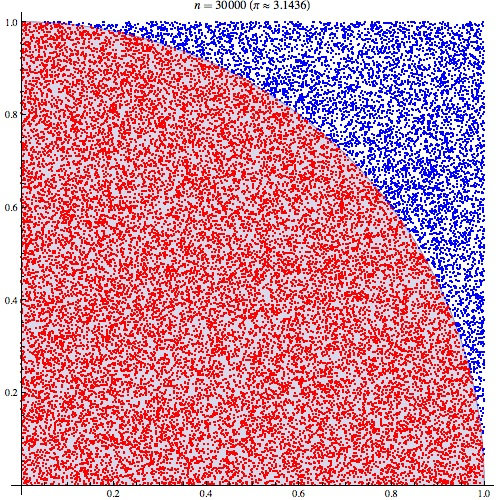
\includegraphics{Pi_30K_1frame.jpg}
\caption{Estimating $\pi$ via random sampling of points. Attribution: By CaitlinJo {[}CC-BY-3.0 (\href{http://creativecommons.org/licenses/by/3.0}{http://creativecommons.org/licenses/by/3.0}){]}, via Wikimedia Commons.}\end{figure}


\strong{See Also:}


\href{http://www.fogcreek.com/fogbugz/evidence-based-scheduling/}{How FogBugz uses Monte Carlo Simulations to estimate the time their software projects will take}




\section{Simulating Card Games for Fun and Profit}
\label{Introduction/Introduction:simulating-card-games-for-fun-and-profit}
The original motivating example that Monte Carlo methods draw their name
from is gambling and game playing. In this module, we develop parallel
algorithms that approximate the probabilities of various outcomes in card
games and the roulette wheel.


\chapter{About Randomness}
\label{Introduction/Introduction:about-randomness}\label{Introduction/Introduction:monte-carlo-methods}

\section{How Computers Generate Random Numbers}
\label{Introduction/Introduction:how-computers-generate-random-numbers}
Algorithms that implement Monte Carlo methods require a source of of
randomness. If we are writing a serial algorithm, we can simply use the
standard random number generator, for example, rand() in C. Computers (unless
specifically fitted with a chip which gathers randomness from some other source)
cannot produce true random numbers. Rather, the standard library random number
generator takes some relatively random 32-bit or 64-bit integer input, called the seed,
and transforms it sequentially
to produce a stream of psuedo-random numbers. A random number generator is created
with the seed as input to a function called \emph{srand()}, and each time a new random number is requested using the \emph{rand()} function, the
integer pattern is changed to produce a new number.  The sequence of numbers produced by such a pseudorandom
number generation algorithm try to approximate a uniform distribution of numbers, each one
statistically independent from the others.

\begin{notice}{note}{Note:}
It is important to realize that a pseudorandom number generator function such
as rand() creates the same sequence of numbers every time for a given input seed, which is typically
a very large integer.  In C and C++, we often use the function time() create the seed integer,
because it returns the number of seconds since January 1, 1970.  When running a sequential
program multiple times, this seed would be different each time the program was run and the pattern
of random numbers generated would be different.
\end{notice}


\chapter{Testing out random number generators: Flip a coin many times}
\label{Introduction/CoinFlip:testing-out-random-number-generators-flip-a-coin-many-times}\label{Introduction/CoinFlip::doc}
A simple way to see how well a random number generator is working is
to simulate flipping a coin over and over again for many trials.

Let's look at some C/C++ code to do this.  The listing below
shows how we can use srand() to seed our random number generator with
a large integer and then make many calls to rand() (or rand\_r() on linux/unix)
to obtain a series
of random integers.  If the integer is even, we call it a `head' coin flip, otherwise
it is a `tail'.  This code sets up trials of coin flips with ever increasing
numbers of flips.  It also calculates the Chi Square statistic using the number of heads
and number of tails.  A rule of thumb in the case of heads and tails is that if the
Chi-Square value is around 3.8 or less, we have a good random distribution of the
even and odd values.  We want to verify that the random number generator provides
such an independent distribution.


\strong{See Also:}


For more details about chi square calculations and how they measure whether a set of values
flows an independent distribution, please see
\href{http://www.radford.edu/~rsheehy/Gen\_flash/Tutorials/Chi-Square\_tutorial/x2-tut.htm}{A Chi-square tutorial},
which shows an example for coin-flipping.

There are many other examples you can find by searching on the web.



In the main() there is a while loop that conducts the trials of coin flips.  Each trial is
conducted by obtaining random numbers in the for loop on line 60.
You can download the file
\code{coinFlip\_seq.cpp} and try this code below yourself.  You should note that the longer trials with many coin flips take a somewhat long time (on the order of 20 seconds, depending on your machine).

In the next section, we will look at parallelizing code using threads and OpenMP, then we will explore how we can conduct the coin-flipping simulation in parallel so that it runs considerably faster.

\begin{Verbatim}[commandchars=\\\{\},numbers=left,firstnumber=1,stepnumber=1]
\PYG{c+cm}{/*}
\PYG{c+cm}{  Original code provided by Dave Valentine, Slippery Rock University.}
\PYG{c+cm}{  Edited by Libby Shoop, Macalester College.}
\PYG{c+cm}{*/}
\PYG{c+c1}{//}
\PYG{c+c1}{// Simulate many coin flips with rand() to determine how}
\PYG{c+c1}{// random the values are that are returned from each call.}
\PYG{c+c1}{//}

\PYG{c+cp}{\PYGZsh{}}\PYG{c+cp}{include \PYGZlt{}stdio.h\PYGZgt{}        }\PYG{c+c1}{// printf()}
\PYG{c+cp}{\PYGZsh{}}\PYG{c+cp}{include \PYGZlt{}stdlib.h\PYGZgt{}       }\PYG{c+c1}{// srand() and rand()}
\PYG{c+cp}{\PYGZsh{}}\PYG{c+cp}{include \PYGZlt{}time.h\PYGZgt{}        }\PYG{c+c1}{// time()}

\PYG{c+c1}{//const int MAX = 1\PYGZlt{}\PYGZlt{}30; //1 gig}

\PYG{c+c1}{//Standard chi sqaure test}
\PYG{k+kt}{double} \PYG{n+nf}{chiSq}\PYG{p}{(}\PYG{k+kt}{int} \PYG{n}{heads}\PYG{p}{,} \PYG{k+kt}{int} \PYG{n}{tails}\PYG{p}{)} \PYG{p}{\PYGZob{}}
    \PYG{k+kt}{double} \PYG{n}{sum} \PYG{o}{=} \PYG{l+m+mi}{0}\PYG{p}{;}					\PYG{c+c1}{//chi square sum}
    \PYG{k+kt}{double} \PYG{n}{tot} \PYG{o}{=} \PYG{n}{heads}\PYG{o}{+}\PYG{n}{tails}\PYG{p}{;}		\PYG{c+c1}{//total flips}
    \PYG{k+kt}{double} \PYG{n}{expected} \PYG{o}{=} \PYG{l+m+mf}{0.5} \PYG{o}{*} \PYG{n}{tot}\PYG{p}{;}	\PYG{c+c1}{//expected heads (or tails)}
    
    \PYG{n}{sum} \PYG{o}{=} \PYG{p}{(}\PYG{p}{(}\PYG{n}{heads} \PYG{o}{-} \PYG{n}{expected}\PYG{p}{)}\PYG{o}{*}\PYG{p}{(}\PYG{n}{heads}\PYG{o}{-}\PYG{n}{expected}\PYG{p}{)}\PYG{o}{/}\PYG{n}{expected}\PYG{p}{)} \PYG{o}{+} \PYGZbs{}
        \PYG{p}{(}\PYG{p}{(}\PYG{n}{tails} \PYG{o}{-} \PYG{n}{expected}\PYG{p}{)}\PYG{o}{*}\PYG{p}{(}\PYG{n}{tails}\PYG{o}{-}\PYG{n}{expected}\PYG{p}{)}\PYG{o}{/}\PYG{n}{expected}\PYG{p}{)}\PYG{p}{;}
    \PYG{k}{return} \PYG{n}{sum}\PYG{p}{;}
\PYG{p}{\PYGZcb{}}


\PYG{k+kt}{int} \PYG{n+nf}{main}\PYG{p}{(}\PYG{p}{)} \PYG{p}{\PYGZob{}}
    \PYG{k+kt}{int} \PYG{n}{numFlips}\PYG{p}{,}			\PYG{c+c1}{//loop control}
        \PYG{n}{numHeads}\PYG{p}{,} \PYG{n}{numTails}\PYG{p}{;}	\PYG{c+c1}{//counters}
        \PYG{k+kt}{clock\PYGZus{}t} \PYG{n}{startTime}\PYG{p}{,} \PYG{n}{stopTime}\PYG{p}{;} \PYG{c+c1}{//wallclock timer}

\PYG{c+cm}{/***** Initialization *****/}

    \PYG{n}{printf}\PYG{p}{(}\PYG{l+s}{"}\PYG{l+s}{Sequential Simulation of Coin Flip using rand()}\PYG{l+s+se}{\PYGZbs{}n}\PYG{l+s}{"}\PYG{p}{)}\PYG{p}{;}
    
    \PYG{c+c1}{//print our heading text}
    \PYG{n}{printf}\PYG{p}{(}\PYG{l+s}{"}\PYG{l+s+se}{\PYGZbs{}n}\PYG{l+s+se}{\PYGZbs{}n}\PYG{l+s}{\PYGZpc{}15s\PYGZpc{}15s\PYGZpc{}15s\PYGZpc{}15s\PYGZpc{}15s\PYGZpc{}15s}\PYG{l+s}{"}\PYG{p}{,}
           \PYG{l+s}{"}\PYG{l+s}{Trials}\PYG{l+s}{"}\PYG{p}{,}\PYG{l+s}{"}\PYG{l+s}{numHeads}\PYG{l+s}{"}\PYG{p}{,}\PYG{l+s}{"}\PYG{l+s}{numTails}\PYG{l+s}{"}\PYG{p}{,}\PYG{l+s}{"}\PYG{l+s}{total}\PYG{l+s}{"}\PYG{p}{,}
           \PYG{l+s}{"}\PYG{l+s}{Chi Squared}\PYG{l+s}{"}\PYG{p}{,} \PYG{l+s}{"}\PYG{l+s}{Time (sec)}\PYG{l+s+se}{\PYGZbs{}n}\PYG{l+s}{"}\PYG{p}{)}\PYG{p}{;}

    \PYG{c+c1}{//create seed using current time}
    \PYG{k+kt}{unsigned} \PYG{k+kt}{int} \PYG{n}{seed} \PYG{o}{=} \PYG{p}{(}\PYG{k+kt}{unsigned}\PYG{p}{)} \PYG{n}{time}\PYG{p}{(}\PYG{n+nb}{NULL}\PYG{p}{)}\PYG{p}{;}
    
    \PYG{c+c1}{//create the pseudorandom number generator}
    \PYG{n}{srand}\PYG{p}{(}\PYG{n}{seed}\PYG{p}{)}\PYG{p}{;}
    
\PYG{c+c1}{// Try several trials of different numbers of flips, doubling how many each round.}
\PYG{c+c1}{// }
\PYG{c+c1}{// Use a unsigned int because we will try a great deal of flips for some trials.}
    \PYG{k+kt}{unsigned} \PYG{k+kt}{int} \PYG{n}{trialFlips} \PYG{o}{=} \PYG{l+m+mi}{256}\PYG{p}{;}       \PYG{c+c1}{// start with a small number of flips}
    \PYG{k+kt}{unsigned} \PYG{k+kt}{int} \PYG{n}{maxFlips} \PYG{o}{=} \PYG{l+m+mi}{1073741824}\PYG{p}{;}  \PYG{c+c1}{// end with a very large number of flips}
    
    \PYG{c+c1}{// below we will double the number of trial flips and come back here}
    \PYG{c+c1}{// and run another trial, until we have reached \PYGZgt{} maxFlips.}
    \PYG{c+c1}{// This will be a total of 23 trials}
    \PYG{k}{while} \PYG{p}{(}\PYG{n}{trialFlips} \PYG{o}{\PYGZlt{}}\PYG{o}{=} \PYG{n}{maxFlips}\PYG{p}{)} \PYG{p}{\PYGZob{}}  
        \PYG{c+c1}{// reset counters for each trial}
        \PYG{n}{numHeads} \PYG{o}{=} \PYG{l+m+mi}{0}\PYG{p}{;}
        \PYG{n}{numTails} \PYG{o}{=} \PYG{l+m+mi}{0}\PYG{p}{;}
        \PYG{n}{startTime} \PYG{o}{=} \PYG{n}{clock}\PYG{p}{(}\PYG{p}{)}\PYG{p}{;}		\PYG{c+c1}{//get start time for this trial}
        
    \PYG{c+cm}{/***** Flip a coin trialFlips times ****/}
        \PYG{k}{for} \PYG{p}{(}\PYG{n}{numFlips}\PYG{o}{=}\PYG{l+m+mi}{0}\PYG{p}{;} \PYG{n}{numFlips}\PYG{o}{\PYGZlt{}}\PYG{n}{trialFlips}\PYG{p}{;} \PYG{n}{numFlips}\PYG{o}{+}\PYG{o}{+}\PYG{p}{)} \PYG{p}{\PYGZob{}}
            \PYG{c+c1}{// if random number is even, call it heads}
            \PYG{c+c1}{// if (rand()\PYGZpc{}2 == 0)     // on Windows, use this}
            \PYG{k}{if} \PYG{p}{(}\PYG{n}{rand\PYGZus{}r}\PYG{p}{(}\PYG{o}{\PYGZam{}}\PYG{n}{seed}\PYG{p}{)}\PYG{o}{\PYGZpc{}}\PYG{l+m+mi}{2} \PYG{o}{=}\PYG{o}{=} \PYG{l+m+mi}{0}\PYG{p}{)} \PYG{c+c1}{// on linux, can use this}
                \PYG{n}{numHeads}\PYG{o}{+}\PYG{o}{+}\PYG{p}{;}
            \PYG{k}{else}
                \PYG{n}{numTails}\PYG{o}{+}\PYG{o}{+}\PYG{p}{;}
        \PYG{p}{\PYGZcb{}}
        
        \PYG{n}{stopTime} \PYG{o}{=} \PYG{n}{clock}\PYG{p}{(}\PYG{p}{)}\PYG{p}{;}   \PYG{c+c1}{// stop the clock}
        
        \PYG{c+cm}{/***** Show the results  for this trial  *****/}
        \PYG{n}{printf}\PYG{p}{(}\PYG{l+s}{"}\PYG{l+s}{\PYGZpc{}15d\PYGZpc{}15d\PYGZpc{}15d\PYGZpc{}15d\PYGZpc{}15.6f\PYGZpc{}15.6f}\PYG{l+s+se}{\PYGZbs{}n}\PYG{l+s}{"}\PYG{p}{,} \PYG{n}{trialFlips}\PYG{p}{,} \PYG{n}{numHeads}\PYG{p}{,} \PYG{n}{numTails}\PYG{p}{,}
               \PYG{p}{(}\PYG{n}{numHeads}\PYG{o}{+}\PYG{n}{numTails}\PYG{p}{)}\PYG{p}{,} \PYG{n}{chiSq}\PYG{p}{(}\PYG{n}{numHeads}\PYG{p}{,} \PYG{n}{numTails}\PYG{p}{)}\PYG{p}{,}
               \PYG{p}{(}\PYG{k+kt}{double}\PYG{p}{)}\PYG{p}{(}\PYG{n}{stopTime}\PYG{o}{-}\PYG{n}{startTime}\PYG{p}{)}\PYG{o}{/}\PYG{n}{CLOCKS\PYGZus{}PER\PYGZus{}SEC}\PYG{p}{)}\PYG{p}{;}

        \PYG{n}{trialFlips} \PYG{o}{*}\PYG{o}{=} \PYG{l+m+mi}{2}\PYG{p}{;}  \PYG{c+c1}{// double the number of flips for the next trial}
    \PYG{p}{\PYGZcb{}}

\PYG{c+cm}{/***** Finish Up *****/}
    \PYG{n}{printf}\PYG{p}{(}\PYG{l+s}{"}\PYG{l+s+se}{\PYGZbs{}n}\PYG{l+s+se}{\PYGZbs{}n}\PYG{l+s+se}{\PYGZbs{}t}\PYG{l+s}{\PYGZlt{}\PYGZlt{}\PYGZlt{} Normal Termination \PYGZgt{}\PYGZgt{}\PYGZgt{}}\PYG{l+s+se}{\PYGZbs{}n}\PYG{l+s+se}{\PYGZbs{}n}\PYG{l+s}{"}\PYG{p}{)}\PYG{p}{;}
    \PYG{k}{return} \PYG{l+m+mi}{0}\PYG{p}{;}
\PYG{p}{\PYGZcb{}}
\end{Verbatim}


\chapter{Parallel Code with Threads}
\label{Threads/Threads_OMP:parallel-code-with-threads}\label{Threads/Threads_OMP::doc}
We can make code that will run our coin flipping simulation faster, by making use of the cores available in multicore CPUs.  We call this type of code parallel code, because we can designate portions of our program to run concurrently in parallel on different cores, computing part of the overall solution.  In the case of flipping a coin, we can intuitively sense that it might be simple enough to designate that each core we have available could carry out some portion of the flips independently while other cores were taking care of the rest of the needed flips.

A common mechanism we use to run code on multiple cores simultaneously is by starting \textbf{threads} that can excute part of our code independently and in parallel on separate cores, sharing data values in memory if needed.  When a program using threads begins execution, it is always running on a single main thread, which we conceptually label as thread 0.  Then within the code we can designate that more threads should start executing in parallel along with thread 0.  We call a point in the code where multiple threads are executing concurrently a \textbf{fork} of those threads.  Then when they are done executing, we think of them as \textbf{joining} back with the main thread. Conceptually, this looks like this:

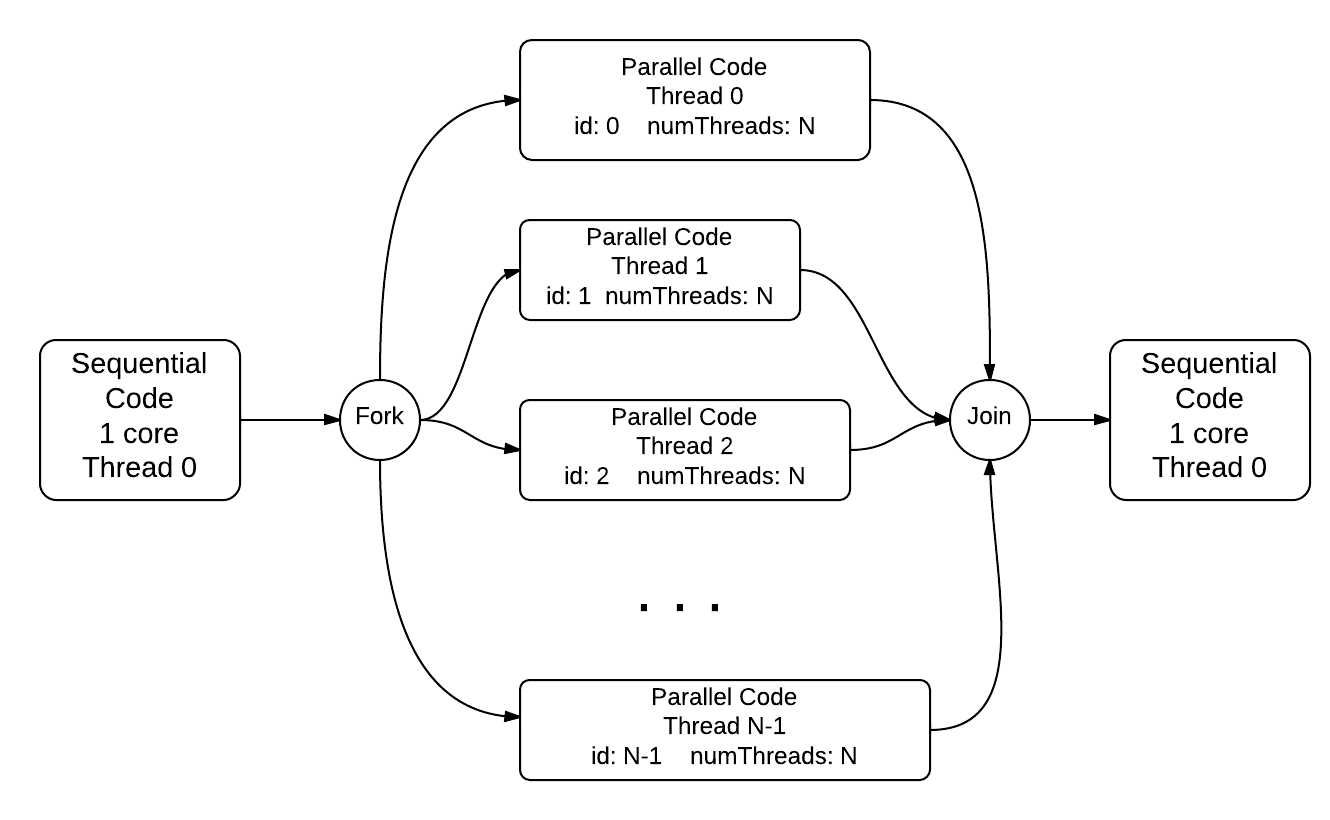
\includegraphics{ForkJoin_SPMD.png}


\section{OpenMP: C/C++ aid for providing threads}
\label{Threads/Threads_OMP:openmp-c-c-aid-for-providing-threads}
The basic library for threading in C/C++ on linux/unix is called \emph{pthreads}.  There are several other thread libraries for other operating systems.  A more convenient way to get started using threads is to use \textbf{OpenMP}, which is built into several popular C/C++ compilers as means to compile high-level directives into threaded code using an underlying threads library.

Let's take a look at a very simple example of how this works:

\begin{Verbatim}[commandchars=\\\{\},numbers=left,firstnumber=1,stepnumber=1]
\PYG{c+cm}{/*}
\PYG{c+cm}{ * Illustration of OpenMP thread forking.}
\PYG{c+cm}{ */}

\PYG{c+cp}{\PYGZsh{}}\PYG{c+cp}{include \PYGZlt{}stdio.h\PYGZgt{}}
\PYG{c+cp}{\PYGZsh{}}\PYG{c+cp}{include \PYGZlt{}omp.h\PYGZgt{}}

\PYG{k+kt}{int} \PYG{n+nf}{main}\PYG{p}{(}\PYG{k+kt}{int} \PYG{n}{argc}\PYG{p}{,} \PYG{k+kt}{char}\PYG{o}{*}\PYG{o}{*} \PYG{n}{argv}\PYG{p}{)} \PYG{p}{\PYGZob{}}
    \PYG{n}{printf}\PYG{p}{(}\PYG{l+s}{"}\PYG{l+s+se}{\PYGZbs{}n}\PYG{l+s}{"}\PYG{p}{)}\PYG{p}{;}

\PYG{c+cp}{\PYGZsh{}}\PYG{c+cp}{pragma omp parallel }
    \PYG{p}{\PYGZob{}}
        \PYG{k+kt}{int} \PYG{n}{id} \PYG{o}{=} \PYG{n}{omp\PYGZus{}get\PYGZus{}thread\PYGZus{}num}\PYG{p}{(}\PYG{p}{)}\PYG{p}{;}
        \PYG{k+kt}{int} \PYG{n}{numThreads} \PYG{o}{=} \PYG{n}{omp\PYGZus{}get\PYGZus{}num\PYGZus{}threads}\PYG{p}{(}\PYG{p}{)}\PYG{p}{;}
        \PYG{n}{printf}\PYG{p}{(}\PYG{l+s}{"}\PYG{l+s}{Hello from thread \PYGZpc{}d of \PYGZpc{}d}\PYG{l+s+se}{\PYGZbs{}n}\PYG{l+s}{"}\PYG{p}{,} \PYG{n}{id}\PYG{p}{,} \PYG{n}{numThreads}\PYG{p}{)}\PYG{p}{;}
    \PYG{p}{\PYGZcb{}}

    \PYG{n}{printf}\PYG{p}{(}\PYG{l+s}{"}\PYG{l+s+se}{\PYGZbs{}n}\PYG{l+s}{"}\PYG{p}{)}\PYG{p}{;}
    \PYG{k}{return} \PYG{l+m+mi}{0}\PYG{p}{;}
\PYG{p}{\PYGZcb{}}
\end{Verbatim}

Line 11 of this code illustrates how we can designate that the main thread 0 should fork and start multiple threads simultaneously. The code within the block following that line and between the curly braces will execute independently on each thread.  Lines 13 and 14 illustrate functions that are available as part of the OpenMP library, which was included on line 6.  There are several other functions available, most notably one that lets you set the number of threads to use, \emph{omp\_set\_num\_threads}, and one that lets you time your threaded code, \emph{omp\_get\_wtime}, to see how much faster it performs.

\begin{notice}{note}{Note:}
When you try an example like this, you should take special note that the order in which each thread will complete \emph{is not guaranteed}.
\end{notice}

\textbf{compiling:} To compile a code file like this in linux/unix, you will need to add this option to gcc or g++ in your makefile or on the command line: \emph{-fopenmp}.  In and IDE like Visual Studio, you will need to set a preference on your project for the C/C++ language to enable OpenMP.


\section{For loop parallelization}
\label{Threads/Threads_OMP:for-loop-parallelization}
In a great deal of code examples, much of the work being performed can be found within for loops that are performing a large number of iterations, such as the coin-flipping example in the previous section.  A well-used pattern in parallel programming is to split the work being done in these loops across multiple forked threads.  OpenMP has a pragma for deisgnating this in the code.  Here is a simple example:

\begin{Verbatim}[commandchars=\\\{\},numbers=left,firstnumber=1,stepnumber=1]
\PYG{c+cm}{/* }
\PYG{c+cm}{ * Parallel for loop using equal chunks per thread.}
\PYG{c+cm}{ */}

\PYG{c+cp}{\PYGZsh{}}\PYG{c+cp}{include \PYGZlt{}stdio.h\PYGZgt{}    }\PYG{c+c1}{// printf()}
\PYG{c+cp}{\PYGZsh{}}\PYG{c+cp}{include \PYGZlt{}stdlib.h\PYGZgt{}   }\PYG{c+c1}{// atoi()}
\PYG{c+cp}{\PYGZsh{}}\PYG{c+cp}{include \PYGZlt{}omp.h\PYGZgt{}      }\PYG{c+c1}{// OpenMP}

\PYG{k+kt}{int} \PYG{n+nf}{main}\PYG{p}{(}\PYG{k+kt}{int} \PYG{n}{argc}\PYG{p}{,} \PYG{k+kt}{char}\PYG{o}{*}\PYG{o}{*} \PYG{n}{argv}\PYG{p}{)} \PYG{p}{\PYGZob{}}
    \PYG{k}{const} \PYG{k+kt}{int} \PYG{n}{REPS} \PYG{o}{=} \PYG{l+m+mi}{16}\PYG{p}{;}

    \PYG{n}{omp\PYGZus{}set\PYGZus{}num\PYGZus{}threads}\PYG{p}{(}\PYG{l+m+mi}{4}\PYG{p}{)}\PYG{p}{;}

    \PYG{c+cp}{\PYGZsh{}}\PYG{c+cp}{pragma omp parallel for  }
    \PYG{k}{for} \PYG{p}{(}\PYG{k+kt}{int} \PYG{n}{i} \PYG{o}{=} \PYG{l+m+mi}{0}\PYG{p}{;} \PYG{n}{i} \PYG{o}{\PYGZlt{}} \PYG{n}{REPS}\PYG{p}{;} \PYG{n}{i}\PYG{o}{+}\PYG{o}{+}\PYG{p}{)} \PYG{p}{\PYGZob{}}
        \PYG{k+kt}{int} \PYG{n}{id} \PYG{o}{=} \PYG{n}{omp\PYGZus{}get\PYGZus{}thread\PYGZus{}num}\PYG{p}{(}\PYG{p}{)}\PYG{p}{;}
        \PYG{n}{printf}\PYG{p}{(}\PYG{l+s}{"}\PYG{l+s}{Thread \PYGZpc{}d performed iteration \PYGZpc{}d}\PYG{l+s+se}{\PYGZbs{}n}\PYG{l+s}{"}\PYG{p}{,} 
                 \PYG{n}{id}\PYG{p}{,} \PYG{n}{i}\PYG{p}{)}\PYG{p}{;}
    \PYG{p}{\PYGZcb{}}

    \PYG{n}{printf}\PYG{p}{(}\PYG{l+s}{"}\PYG{l+s}{Main thread 0 done.}\PYG{l+s+se}{\PYGZbs{}n}\PYG{l+s}{"}\PYG{p}{)}\PYG{p}{;}
    \PYG{k}{return} \PYG{l+m+mi}{0}\PYG{p}{;}
\PYG{p}{\PYGZcb{}}
\end{Verbatim}

In this example, we set up a very small number of repetitions of the loop, simply to illustrate how forking threads and running the loop iterations works.  The OpenMP pragma on line 14 is asking the compiler to set up an equal distribution of work for each thread, which will take place like this for the 4 threads indicated on line 12 and the 16 repetitions of the for loop:

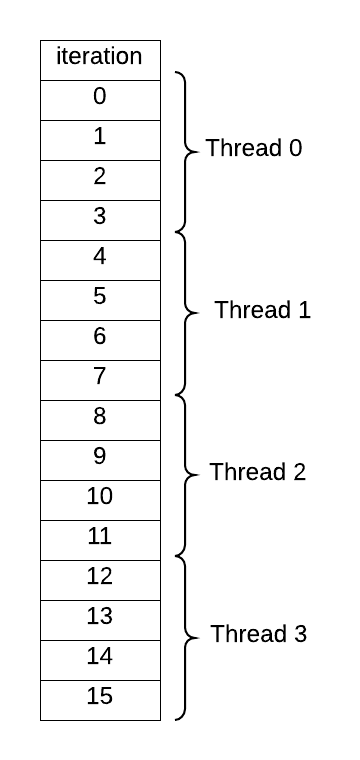
\includegraphics{ParalleFor_Chunks-4_threads.png}

When running a simple example like this, you will find that each repetition will not be carried out in order from 0 through 15, as each thread will do its designated repetitions at the same time as the other threads, shceduled by the operating system on the cores available.


\section{Next step: using OpenMP}
\label{Threads/Threads_OMP:next-step-using-openmp}
In the next section we will see how we can use threads and OpenMP to make coin flipping faster.


\chapter{Coin-flipping in Parallel}
\label{Threads/OpenMP_CoinFlip:coin-flipping-in-parallel}\label{Threads/OpenMP_CoinFlip::doc}
Now that we know a bit about how OpenMP works to provide threads that run code in parallel, let's look at how we can update our coin-flipping example.
The places in this code where you see this comment:

\begin{Verbatim}[commandchars=\\\{\}]
    \PYG{c+cm}{/***  OMP ***/}
\end{Verbatim}

indicate where OpenMP was used to enable running the original coin-flipping code example on multiple threads, or where the code needed changes to enable running on multiple threads.  Examine these places in the following code:

\begin{Verbatim}[commandchars=\\\{\},numbers=left,firstnumber=1,stepnumber=1]
\PYG{c+cm}{/*}
\PYG{c+cm}{  Original code provided by Dave Valentine, Slippery Rock University.}
\PYG{c+cm}{  Edited by Libby Shoop, Macalester College.}
\PYG{c+cm}{*/}
\PYG{c+c1}{//}
\PYG{c+c1}{// Simulate many coin flips with rand\PYGZus{}r() on multiple threads}
\PYG{c+c1}{// to determine how random the values are that are returned}
\PYG{c+c1}{// from each call.}
\PYG{c+c1}{//}

\PYG{c+cp}{\PYGZsh{}}\PYG{c+cp}{include \PYGZlt{}stdio.h\PYGZgt{}        }\PYG{c+c1}{// printf()}
\PYG{c+cp}{\PYGZsh{}}\PYG{c+cp}{include \PYGZlt{}stdlib.h\PYGZgt{}       }\PYG{c+c1}{// srand() and rand()}
\PYG{c+cp}{\PYGZsh{}}\PYG{c+cp}{include \PYGZlt{}time.h\PYGZgt{}         }\PYG{c+c1}{// time()}

\PYG{c+cp}{\PYGZsh{}}\PYG{c+cp}{include \PYGZlt{}omp.h\PYGZgt{}          }\PYG{c+c1}{// OpenMP functions and pragmas}


\PYG{c+c1}{//Standard chi sqaure test}
\PYG{k+kt}{double} \PYG{n+nf}{chiSq}\PYG{p}{(}\PYG{k+kt}{int} \PYG{n}{heads}\PYG{p}{,} \PYG{k+kt}{int} \PYG{n}{tails}\PYG{p}{)} \PYG{p}{\PYGZob{}}
    \PYG{k+kt}{double} \PYG{n}{sum} \PYG{o}{=} \PYG{l+m+mi}{0}\PYG{p}{;}                \PYG{c+c1}{//chi square sum}
    \PYG{k+kt}{double} \PYG{n}{tot} \PYG{o}{=} \PYG{n}{heads}\PYG{o}{+}\PYG{n}{tails}\PYG{p}{;}      \PYG{c+c1}{//total flips}
    \PYG{k+kt}{double} \PYG{n}{expected} \PYG{o}{=} \PYG{l+m+mf}{0.5} \PYG{o}{*} \PYG{n}{tot}\PYG{p}{;}   \PYG{c+c1}{//expected heads (or tails)}
    
    \PYG{n}{sum} \PYG{o}{=} \PYG{p}{(}\PYG{p}{(}\PYG{n}{heads} \PYG{o}{-} \PYG{n}{expected}\PYG{p}{)}\PYG{o}{*}\PYG{p}{(}\PYG{n}{heads}\PYG{o}{-}\PYG{n}{expected}\PYG{p}{)}\PYG{o}{/}\PYG{n}{expected}\PYG{p}{)} \PYG{o}{+} \PYGZbs{}
        \PYG{p}{(}\PYG{p}{(}\PYG{n}{tails} \PYG{o}{-} \PYG{n}{expected}\PYG{p}{)}\PYG{o}{*}\PYG{p}{(}\PYG{n}{tails}\PYG{o}{-}\PYG{n}{expected}\PYG{p}{)}\PYG{o}{/}\PYG{n}{expected}\PYG{p}{)}\PYG{p}{;}
    \PYG{k}{return} \PYG{n}{sum}\PYG{p}{;}
\PYG{p}{\PYGZcb{}}



\PYG{k+kt}{int} \PYG{n+nf}{main}\PYG{p}{(}\PYG{p}{)} \PYG{p}{\PYGZob{}}
    \PYG{k+kt}{int} \PYG{n}{numFlips}\PYG{p}{,}             \PYG{c+c1}{//loop control}
        \PYG{n}{numHeads}\PYG{p}{,} \PYG{n}{numTails}\PYG{p}{;}   \PYG{c+c1}{//counters}
    
    \PYG{c+cm}{/***  OMP ***/}
    \PYG{k+kt}{int} \PYG{n}{nThreads}\PYG{p}{;}           \PYG{c+c1}{// number of threads to use}
    \PYG{k+kt}{double} \PYG{n}{ompStartTime}\PYG{p}{,} \PYG{n}{ompStopTime}\PYG{p}{;}  \PYG{c+c1}{// holds wall clock time}
    \PYG{c+cm}{/***  OMP ***/}


\PYG{c+cm}{/***** Initialization *****/}
    
    \PYG{n}{printf}\PYG{p}{(}\PYG{l+s}{"}\PYG{l+s}{Threaded Simulation of Coin Flip using rand\PYGZus{}r()}\PYG{l+s+se}{\PYGZbs{}n}\PYG{l+s}{"}\PYG{p}{)}\PYG{p}{;}
    \PYG{c+cm}{/***  OMP ***/}
    \PYG{n}{nThreads} \PYG{o}{=} \PYG{l+m+mi}{4}\PYG{p}{;}     \PYG{c+c1}{// try increasing this if you have more cores}
    
    \PYG{c+c1}{//print our heading text}
    \PYG{n}{printf}\PYG{p}{(}\PYG{l+s}{"}\PYG{l+s+se}{\PYGZbs{}n}\PYG{l+s+se}{\PYGZbs{}n}\PYG{l+s}{\PYGZpc{}15s\PYGZpc{}15s\PYGZpc{}15s\PYGZpc{}15s\PYGZpc{}15s\PYGZpc{}15s}\PYG{l+s}{"}\PYG{p}{,}
           \PYG{l+s}{"}\PYG{l+s}{Trials}\PYG{l+s}{"}\PYG{p}{,}\PYG{l+s}{"}\PYG{l+s}{numHeads}\PYG{l+s}{"}\PYG{p}{,}\PYG{l+s}{"}\PYG{l+s}{numTails}\PYG{l+s}{"}\PYG{p}{,}\PYG{l+s}{"}\PYG{l+s}{total}\PYG{l+s}{"}\PYG{p}{,}
           \PYG{l+s}{"}\PYG{l+s}{Chi Squared}\PYG{l+s}{"}\PYG{p}{,} \PYG{l+s}{"}\PYG{l+s}{Time (sec)}\PYG{l+s+se}{\PYGZbs{}n}\PYG{l+s}{"}\PYG{p}{)}\PYG{p}{;}
    
    
    \PYG{c+c1}{//create seed using current time}
    \PYG{k+kt}{unsigned} \PYG{k+kt}{int} \PYG{n}{seed} \PYG{o}{=} \PYG{p}{(}\PYG{k+kt}{unsigned}\PYG{p}{)} \PYG{n}{time}\PYG{p}{(}\PYG{n+nb}{NULL}\PYG{p}{)}\PYG{p}{;}
    
    \PYG{c+c1}{//create the pseudorandom number generator}
    \PYG{n}{srand}\PYG{p}{(}\PYG{n}{seed}\PYG{p}{)}\PYG{p}{;}


\PYG{c+c1}{// Try several trials of different numbers of flips doubling how many each round.}
\PYG{c+c1}{// }
\PYG{c+c1}{// Use a unsigned int because we will try a great deal of flips for some trials.}
    \PYG{k+kt}{unsigned} \PYG{k+kt}{int} \PYG{n}{trialFlips} \PYG{o}{=} \PYG{l+m+mi}{256}\PYG{p}{;}          \PYG{c+c1}{// start with a smal number of flips}
    \PYG{k+kt}{unsigned} \PYG{k+kt}{int} \PYG{n}{maxFlips} \PYG{o}{=} \PYG{l+m+mi}{1073741824}\PYG{p}{;}     \PYG{c+c1}{// end with a very large number of flips}
    
    \PYG{c+c1}{// below we will double the number of trial flips and come back here}
    \PYG{c+c1}{// and run another trial, until we have reached \PYGZgt{} maxFlips.}
    \PYG{c+c1}{// This will be a total of 23 trials}
    \PYG{k}{while} \PYG{p}{(}\PYG{n}{trialFlips} \PYG{o}{\PYGZlt{}}\PYG{o}{=} \PYG{n}{maxFlips}\PYG{p}{)} \PYG{p}{\PYGZob{}}  
        
        \PYG{n}{numHeads} \PYG{o}{=} \PYG{l+m+mi}{0}\PYG{p}{;}               \PYG{c+c1}{//reset counters}
        \PYG{n}{numTails} \PYG{o}{=} \PYG{l+m+mi}{0}\PYG{p}{;}
        
        \PYG{c+cm}{/***  OMP ***/}
        \PYG{n}{ompStartTime} \PYG{o}{=} \PYG{n}{omp\PYGZus{}get\PYGZus{}wtime}\PYG{p}{(}\PYG{p}{)}\PYG{p}{;}   \PYG{c+c1}{//get start time for this trial}
    
    \PYG{c+cm}{/***** Flip a coin trialFlips times, on each thread in parallel,}
\PYG{c+cm}{     *     with each thread getting its 1/4 share of the total flips.}
\PYG{c+cm}{     *****/}

\PYG{c+cm}{/***  OMP ***/}
\PYG{c+cp}{\PYGZsh{}}\PYG{c+cp}{pragma omp parallel for num\PYGZus{}threads(nThreads) default(none) \PYGZbs{}}
\PYG{c+cp}{        private(numFlips, seed) \PYGZbs{}}
\PYG{c+cp}{        shared(trialFlips) \PYGZbs{}}
\PYG{c+cp}{        reduction(+:numHeads, numTails)}
        \PYG{k}{for} \PYG{p}{(}\PYG{n}{numFlips}\PYG{o}{=}\PYG{l+m+mi}{0}\PYG{p}{;} \PYG{n}{numFlips}\PYG{o}{\PYGZlt{}}\PYG{n}{trialFlips}\PYG{p}{;} \PYG{n}{numFlips}\PYG{o}{+}\PYG{o}{+}\PYG{p}{)} \PYG{p}{\PYGZob{}}
            \PYG{c+c1}{// rand() is not thread safe in linux}
            \PYG{c+c1}{// rand\PYGZus{}r() is available in linux and thread safe,}
            \PYG{c+c1}{// to be run on separate threads concurrently.}
            \PYG{c+c1}{// On windows in visual studio, use rand(), which is thread safe.}
            \PYG{k}{if} \PYG{p}{(}\PYG{n}{rand\PYGZus{}r}\PYG{p}{(}\PYG{o}{\PYGZam{}}\PYG{n}{seed}\PYG{p}{)}\PYG{o}{\PYGZpc{}}\PYG{l+m+mi}{2} \PYG{o}{=}\PYG{o}{=} \PYG{l+m+mi}{0}\PYG{p}{)} \PYG{c+c1}{// if random number is even, call it heads}
                \PYG{n}{numHeads}\PYG{o}{+}\PYG{o}{+}\PYG{p}{;}       
            \PYG{k}{else}
                \PYG{n}{numTails}\PYG{o}{+}\PYG{o}{+}\PYG{p}{;}
        \PYG{p}{\PYGZcb{}}
                
        \PYG{c+cm}{/***  OMP ***/}
        \PYG{n}{ompStopTime} \PYG{o}{=} \PYG{n}{omp\PYGZus{}get\PYGZus{}wtime}\PYG{p}{(}\PYG{p}{)}\PYG{p}{;}  \PYG{c+c1}{//get time this trial finished}
        
        \PYG{c+c1}{// Finish this trial by printing out results}

        \PYG{n}{printf}\PYG{p}{(}\PYG{l+s}{"}\PYG{l+s}{\PYGZpc{}15d\PYGZpc{}15d\PYGZpc{}15d\PYGZpc{}15d\PYGZpc{}15.6f\PYGZpc{}15.6f}\PYG{l+s+se}{\PYGZbs{}n}\PYG{l+s}{"}\PYG{p}{,} \PYG{n}{trialFlips}\PYG{p}{,} \PYG{n}{numHeads}\PYG{p}{,} \PYG{n}{numTails}\PYG{p}{,}
               \PYG{p}{(}\PYG{n}{numHeads}\PYG{o}{+}\PYG{n}{numTails}\PYG{p}{)}\PYG{p}{,} \PYG{n}{chiSq}\PYG{p}{(}\PYG{n}{numHeads}\PYG{p}{,} \PYG{n}{numTails}\PYG{p}{)}\PYG{p}{,}
               \PYG{p}{(}\PYG{k+kt}{double}\PYG{p}{)}\PYG{p}{(}\PYG{n}{ompStopTime}\PYG{o}{-}\PYG{n}{ompStartTime}\PYG{p}{)}\PYG{p}{)}\PYG{p}{;}    \PYG{c+cm}{/***  OMP ***/}

        \PYG{n}{trialFlips} \PYG{o}{*}\PYG{o}{=} \PYG{l+m+mi}{2}\PYG{p}{;}   \PYG{c+c1}{// double the number of flips for the next trial}
    \PYG{p}{\PYGZcb{}}
    
    \PYG{c+cm}{/***** Finish Up *****/}
    \PYG{n}{printf}\PYG{p}{(}\PYG{l+s}{"}\PYG{l+s+se}{\PYGZbs{}n}\PYG{l+s+se}{\PYGZbs{}n}\PYG{l+s+se}{\PYGZbs{}t}\PYG{l+s}{\PYGZlt{}\PYGZlt{}\PYGZlt{} Normal Termination \PYGZgt{}\PYGZgt{}\PYGZgt{}}\PYG{l+s+se}{\PYGZbs{}n}\PYG{l+s+se}{\PYGZbs{}n}\PYG{l+s}{"}\PYG{p}{)}\PYG{p}{;}
    \PYG{k}{return} \PYG{l+m+mi}{0}\PYG{p}{;}
\PYG{p}{\PYGZcb{}}
\end{Verbatim}


\section{Some notes about this code}
\label{Threads/OpenMP_CoinFlip:some-notes-about-this-code}\begin{enumerate}
\item {} 
On line 15 we include the OpenMP library.

\item {} 
On lines 75 and 98 we use the OpenMP function to return a wall clock time in seconds.  The difference between these provides the total amount of time to run the section of code enclosed by these lines.  Note that this OpenMP function called \emph{omp\_get\_wtime} specifically provides the overall time for the threaded code to run.  We need to use this function because the original method using the clock() function does not work properly with threaded code.

\item {} 
Lines 82 - 85 indicate the setup for running the for loop of coin flips in equal numbers of iterations per thread. There are several directives needed to be added to the parallel for pragma:
\begin{itemize}
\item {} 
\emph{num\_threads(nThreads)} designates how many threads to fork for this loop.

\item {} 
\emph{default(none)} designates that all variables in the loop will be defined as either private within each thread or shared between the threads by the next three directives.

\item {} 
the \textbackslash{} designates that the pragma declaration is continuing onto another line

\item {} 
\emph{private(numFlips, seed)} designates that each thread will keep its own private copy of the variables numFlips and seed and update them independently.

\item {} 
\emph{shared(trialFlips)} designates that the variable trialFlips is shared by all of the threads (this is safe because no thread will ever update it.)

\item {} 
\emph{reduction(+:numHeads, numTails)} is a special indicator for the the two values numHeads and numTails, which need to get updated by all the threads simultaneously.  Since this will cause errors when the threads are executing, typically the OpenMP threaded code will have each thread keep a private copy of these variables while they execute their portion of the loop.  Then when they join back after they have finished , each thread's private numHeads and numTails sum is added to an overall sum and stored in thread 0's copy of numHeads and numTails.

\end{itemize}

\item {} 
You can download the file \code{coinFlip\_omp.cpp} and try this code  yourself.  If you have 4 cores available on your computer, you should see the longer trials with many coin flips run almost four times faster than our earlier sequential version that did not use threads.

\end{enumerate}
\begin{figure}[htbp]
\centering
\capstart

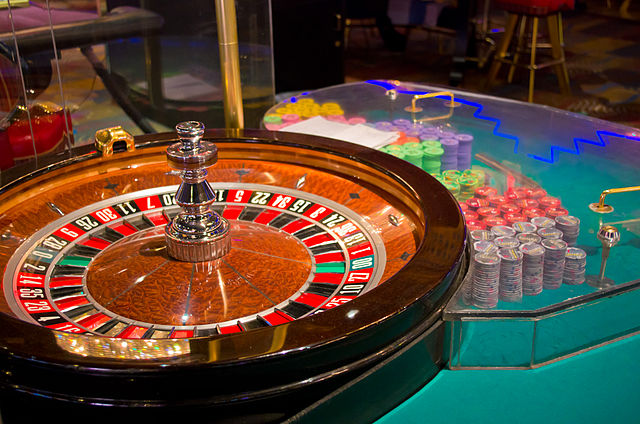
\includegraphics{640px-Sahara_Hotel_and_Casino_2.jpg}
\caption{``Sahara Hotel and Casino 2'' by Antoine Taveneaux - Own work. Licensed under Creative Commons
Attribution-Share Alike 3.0 via
\href{http://commons.wikimedia.org/wiki/File:Sahara\_Hotel\_and\_Casino\_2.jpg\#mediaviewer/File:Sahara\_Hotel\_and\_Casino\_2.jpg}{Wikimedia Commons}}\end{figure}


\chapter{Roulette Simulation}
\label{RouletteSimulation/RouletteSimulation::doc}\label{RouletteSimulation/RouletteSimulation:roulette-simulation}
An American Roulette wheel has 38 slots: 18 are red, 18 are black, and 2 are
green, which the house always wins. When a person bets on either red or black,
the odds of winning are 18/38, or 47.37\% of the time.

Our next is example is a simulation of spinning the Roulette wheel. We have a
main simulation loop that is similar to the coin-flipping example. The code
for determining a win on each spin is more involved than flipping a coin, and
the sequential version,
\code{rouletteSimulation\_seq.cpp}
is decomposed into several methods. Look at this original code file to see how
we run the simulations using increasing numbers of random spins of the wheel.

The function that actually runs a single simulation of the Roulette wheel, called spinRed(),  is quite
simple. It generates a random number to represent the slot that the ball
ends up in and gives a payout according to the rules of Roulette.

\begin{Verbatim}[commandchars=\\\{\}]
\PYG{c+c1}{//spin the wheel, betting on RED}
\PYG{c+c1}{//Payout Rules:}
\PYG{c+c1}{//  0..17 you win (it was red)}
\PYG{c+c1}{// 18..35 you lose (it was black)}
\PYG{c+c1}{// 36..37 house wins (green) - you lose half}
\PYG{k+kt}{int} \PYG{n}{spinRed}\PYG{p}{(}\PYG{k+kt}{int} \PYG{n}{bet}\PYG{p}{,} \PYG{k+kt}{unsigned} \PYG{k+kt}{int} \PYG{o}{*}\PYG{n}{seed}\PYG{p}{)} \PYG{p}{\PYGZob{}}
	\PYG{k+kt}{int} \PYG{n}{payout}\PYG{p}{;}
	\PYG{k+kt}{int} \PYG{n}{slot} \PYG{o}{=} \PYG{n}{rand\PYGZus{}rIntBetween}\PYG{p}{(}\PYG{l+m+mi}{1}\PYG{p}{,}\PYG{l+m+mi}{38}\PYG{p}{,} \PYG{n}{seed}\PYG{p}{)}\PYG{p}{;}
	\PYG{c+cm}{/* if Windows}
\PYG{c+cm}{	int slot = randIntBetween(1,38);}
\PYG{c+cm}{	 */}
	\PYG{k}{if} \PYG{p}{(}\PYG{n}{slot} \PYG{o}{\PYGZlt{}}\PYG{o}{=} \PYG{l+m+mi}{18}\PYG{p}{)} \PYG{c+c1}{//simplify odds: [0..17]==RED}
		\PYG{n}{payout} \PYG{o}{=} \PYG{n}{bet}\PYG{p}{;}	\PYG{c+c1}{//won}
	\PYG{k}{else} \PYG{k}{if} \PYG{p}{(}\PYG{n}{slot} \PYG{o}{\PYGZlt{}}\PYG{o}{=} \PYG{l+m+mi}{36}\PYG{p}{)} \PYG{c+c1}{//spin was 'black'-lose all}
		\PYG{n}{payout} \PYG{o}{=} \PYG{o}{-}\PYG{n}{bet}\PYG{p}{;}	\PYG{c+c1}{//lost}
	\PYG{k}{else} \PYG{c+c1}{//spin was green - lose half}
		\PYG{n}{payout} \PYG{o}{=} \PYG{o}{-}\PYG{p}{(}\PYG{n}{bet}\PYG{o}{/}\PYG{l+m+mi}{2}\PYG{p}{)}\PYG{p}{;} \PYG{c+c1}{//half-back}
	\PYG{k}{return} \PYG{n}{payout}\PYG{p}{;}
\PYG{p}{\PYGZcb{}} \PYG{c+c1}{// spinRed}
\end{Verbatim}

\begin{notice}{note}{Note:}
The sequential version of the simulation takes a fair amount of time. Note how long.
Also note how many simulated random spins it takes before the distribution of spins
accurately reflects the house odds.
\end{notice}


\section{Parallelism to the Rescue}
\label{RouletteSimulation/RouletteSimulation:parallelism-to-the-rescue}
We add OpenMP parallelism as in the coinFlip example, by running the loop of random spins
for each trial on several threads. This code is in this file that you can download:
\code{rouletteSimulation\_omp.cpp}
The actual simulation function is getNumWins():

\begin{Verbatim}[commandchars=\\\{\}]
\PYG{c+cm}{/*********************** getNumWins ************/} 
\PYG{k+kt}{int} \PYG{n}{getNumWins}\PYG{p}{(}\PYG{k+kt}{int} \PYG{n}{numSpins}\PYG{p}{,} \PYG{k+kt}{unsigned} \PYG{k+kt}{int} \PYG{n}{seed}\PYG{p}{)} \PYG{p}{\PYGZob{}}
\PYG{c+c1}{//always bet 'red' \PYGZam{} count wins}
	\PYG{k}{static} \PYG{k+kt}{int} \PYG{n}{wins}\PYG{p}{;}\PYG{c+c1}{//our counter}
	\PYG{k+kt}{int} \PYG{n}{spin}\PYG{p}{;}		\PYG{c+c1}{//loop cntrl var}
	\PYG{k+kt}{int} \PYG{n}{myBet} \PYG{o}{=} \PYG{l+m+mi}{10}\PYG{p}{;} \PYG{c+c1}{//amount we bet per spin}

	\PYG{n}{wins} \PYG{o}{=} \PYG{l+m+mi}{0}\PYG{p}{;}	\PYG{c+c1}{//clear our counter}
	
\PYG{c+cm}{/***  OMP ***/}    
\PYG{c+cp}{\PYGZsh{}}\PYG{c+cp}{pragma omp parallel for num\PYGZus{}threads(nThreads) default(none) \PYGZbs{}}
\PYG{c+cp}{    shared(numSpins, myBet) \PYGZbs{}}
\PYG{c+cp}{	private(spin, seed) \PYGZbs{}}
\PYG{c+cp}{	reduction(+:wins)}
	\PYG{k}{for} \PYG{p}{(}\PYG{n}{spin}\PYG{o}{=}\PYG{l+m+mi}{0}\PYG{p}{;} \PYG{n}{spin}\PYG{o}{\PYGZlt{}}\PYG{n}{numSpins}\PYG{p}{;} \PYG{n}{spin}\PYG{o}{+}\PYG{o}{+}\PYG{p}{)}\PYG{p}{\PYGZob{}}
		\PYG{c+c1}{//spinRed returns +/- number (win/lose)}
		\PYG{k}{if} \PYG{p}{(}\PYG{n}{spinRed}\PYG{p}{(}\PYG{n}{myBet}\PYG{p}{,} \PYG{o}{\PYGZam{}}\PYG{n}{seed}\PYG{p}{)} \PYG{o}{\PYGZgt{}} \PYG{l+m+mi}{0}\PYG{p}{)} \PYG{c+c1}{//a winner!}
			\PYG{n}{wins}\PYG{o}{+}\PYG{o}{+}\PYG{p}{;}
	\PYG{p}{\PYGZcb{}}	\PYG{c+c1}{////  end forked parallel threads}
	
	\PYG{k}{return} \PYG{n}{wins}\PYG{p}{;}
\PYG{p}{\PYGZcb{}}  \PYG{c+c1}{//getNumWins}
\end{Verbatim}

Notes about this code: numSpins and myBet are shared
between threads while spin is the loop index and unique to each thread.
When using rand\_r() as the thread-safe random number generator in linux/unix,
the seed should be private to each thread also.
Like the previous example, we combine the partial results from each
thread with \emph{reduction(+:wins)}.


\chapter{Drawing Four Cards of the Same Suit}
\label{DrawFourSuitsExample/DrawFourSuitsExample:drawing-four-cards-of-the-same-suit}\label{DrawFourSuitsExample/DrawFourSuitsExample::doc}
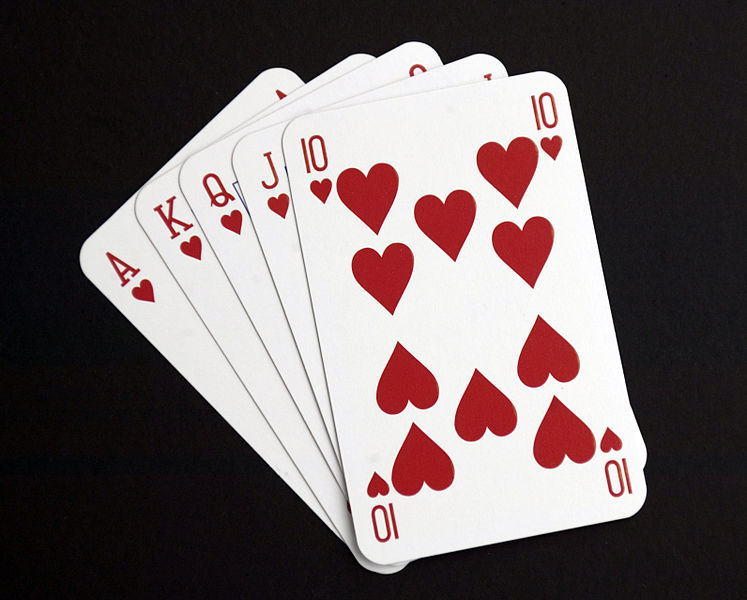
\includegraphics{RoyalFlush.jpg}

Now let's turn our attention to the card game of Poker.
There are methods to calculate the probability of drawing the various types of hands (see the \href{http://en.wikipedia.org/wiki/Poker\_probability}{Wikipedia Poker Probability Page} for explanation).
For our next example, we will examine one such type of hand with the following question:

\emph{If you are dealt a random hand of 5 cards, what is the probability that four of the cards each have a different
suit?}

To answer this question, we simulate shuffling a deck of cards and drawing a hand of cards.


\section{Code Files}
\label{DrawFourSuitsExample/DrawFourSuitsExample:code-files}
For this code, we have separate versions for Windows, which uses rand(), and linux, which uses rand\_r() as the random number generators.

\begin{tabulary}{\linewidth}{|L|L|}
\hline
\textbf{
Linux
} & \textbf{}\\\hline

sequential version:
 & 
\code{drawFourSuits\_seq.cpp}
\\\hline

OpenMP version:
 & 
\code{drawFourSuits\_omp.cpp}
\\\hline
\end{tabulary}


\begin{tabulary}{\linewidth}{|L|L|}
\hline
\textbf{
Windows
} & \textbf{}\\\hline

sequential version:
 & 
\code{drawFourSuits\_seq.cpp}
\\\hline

OpenMP version:
 & 
\code{drawFourSuits\_omp.cpp}
\\\hline
\end{tabulary}



\section{Sequential code}
\label{DrawFourSuitsExample/DrawFourSuitsExample:sequential-code}
We represent the deck of cards as an array of integers. Our function for simulating
deck shuffling is not the most efficient, but it tries to capture how a traditional
``fan'' shuffle actually works. We also have helper functions for initializing a deck,
drawing a hand, and checking if the hand has four cards of the same suit. Download the
appropriate sequential code file for your environment and study it.  Note all the places
where random numbers are generated for two aspects of the problem: shuffling the deck and
picking cards from the deck to form a hand.

Using these helper functions, it was straightforward to write testOneHand,
which initializes a deck, shuffles it, draws a hand, and then checks if
all four suits are represented.

\begin{Verbatim}[commandchars=\\\{\}]
\PYG{c+cm}{/************************************************}
\PYG{c+cm}{***************************** testOneHand *********/}
\PYG{k+kt}{bool} \PYG{n}{testOneHand}\PYG{p}{(}\PYG{k+kt}{unsigned} \PYG{k+kt}{int} \PYG{o}{*}\PYG{n}{seed\PYGZus{}ptr}\PYG{p}{)}\PYG{p}{\PYGZob{}}
\PYG{c+c1}{//Create a deck...sort it...pick 4 cards...test 4 suits}
	\PYG{k+kt}{int} \PYG{n}{deck}\PYG{p}{[}\PYG{n}{MAX\PYGZus{}CARDS}\PYG{p}{]}\PYG{p}{;}	\PYG{c+c1}{//std deck}
	\PYG{k+kt}{int} \PYG{n}{hand}\PYG{p}{[}\PYG{n}{CARDS\PYGZus{}IN\PYGZus{}HAND}\PYG{p}{]}\PYG{p}{;}	\PYG{c+c1}{//card hand}
	
	\PYG{n}{initDeck}\PYG{p}{(}\PYG{n}{deck}\PYG{p}{,} \PYG{n}{seed\PYGZus{}ptr}\PYG{p}{)}\PYG{p}{;}	\PYG{c+c1}{//create \PYGZam{} shuffle a new deck}
	
	\PYG{n}{drawHand}\PYG{p}{(}\PYG{n}{deck}\PYG{p}{,} \PYG{n}{hand}\PYG{p}{,} \PYG{n}{seed\PYGZus{}ptr}\PYG{p}{)}\PYG{p}{;}	\PYG{c+c1}{//go pick cards from deck}
	
	\PYG{k}{return} \PYG{n}{isFourSuits}\PYG{p}{(}\PYG{n}{hand}\PYG{p}{)}\PYG{p}{;} \PYG{c+c1}{//test if 4 suits}
\PYG{p}{\PYGZcb{}}\PYG{c+c1}{//testOneHand}
\end{Verbatim}


\section{Open MP Version}
\label{DrawFourSuitsExample/DrawFourSuitsExample:open-mp-version}
Converting our sequential code to use OpenMP is quite simple. We add a pragma
compiler directive to the main simulation loop to run the loop simultaneously
on multiple CPUs. The directive tells OpenMP to give each thread a different
copy of i since each thread needs to keep track of its own loop iterations.
numTests is shared because the total number of tests to run is doubled only
once per iteration of the out while loop. (If each thread doubled it, we would
go up by more than a factor of two.) Finally, the directive \emph{reduction (+:total)}
tells OpenMP to combine each of the threads' partial results by summing to find
the total number of hands that contained all four suits.

\begin{Verbatim}[commandchars=\\\{\}]
\PYG{c+cm}{/************************* 2.0 Simulation Loop **/}
	\PYG{k}{while} \PYG{p}{(}\PYG{n}{numTests} \PYG{o}{\PYGZlt{}} \PYG{n}{MAX}\PYG{p}{)} \PYG{p}{\PYGZob{}}
		\PYG{n}{total} \PYG{o}{=} \PYG{l+m+mi}{0}\PYG{p}{;}	\PYG{c+c1}{//reset counter}
		
\PYG{c+cp}{\PYGZsh{}}\PYG{c+cp}{pragma omp parallel for num\PYGZus{}threads(nThreads) default(none) \PYGZbs{}}
\PYG{c+cp}{		private (i, seed) \PYGZbs{}}
\PYG{c+cp}{		shared (numTests) \PYGZbs{}}
\PYG{c+cp}{		reduction (+:total)	\PYGZbs{}}
\PYG{c+cp}{		schedule(dynamic)}
		\PYG{k}{for} \PYG{p}{(}\PYG{n}{i}\PYG{o}{=}\PYG{l+m+mi}{0}\PYG{p}{;} \PYG{n}{i}\PYG{o}{\PYGZlt{}}\PYG{n}{numTests}\PYG{p}{;} \PYG{n}{i}\PYG{o}{+}\PYG{o}{+}\PYG{p}{)} \PYG{p}{\PYGZob{}} \PYG{c+c1}{//make new deck - pick hand - test for 4 suits}
			\PYG{k}{if} \PYG{p}{(}\PYG{n}{testOneHand}\PYG{p}{(}\PYG{o}{\PYGZam{}}\PYG{n}{seed}\PYG{p}{)}\PYG{p}{)}		\PYG{c+c1}{//returns TRUE iff 4-suits hand}
				\PYG{n}{total} \PYG{o}{+}\PYG{o}{+}\PYG{p}{;}		\PYG{c+c1}{//tally hands with 4-suits}
		\PYG{p}{\PYGZcb{}}
		\PYG{c+c1}{//calc \PYGZpc{} of 4-suit hands \PYGZam{} report results...}
		\PYG{n}{percentage} \PYG{o}{=} \PYG{l+m+mf}{100.0}\PYG{o}{*}\PYG{p}{(} \PYG{p}{(}\PYG{k+kt}{double}\PYG{p}{)}\PYG{n}{total}\PYG{p}{)}\PYG{o}{/}\PYG{n}{numTests}\PYG{p}{;}
		\PYG{n}{cout}\PYG{o}{\PYGZlt{}}\PYG{o}{\PYGZlt{}}\PYG{n}{setw}\PYG{p}{(}\PYG{l+m+mi}{12}\PYG{p}{)}\PYG{o}{\PYGZlt{}}\PYG{o}{\PYGZlt{}}\PYG{n}{numTests}\PYG{o}{\PYGZlt{}}\PYG{o}{\PYGZlt{}}\PYG{n}{setw}\PYG{p}{(}\PYG{l+m+mi}{14}\PYG{p}{)}\PYG{o}{\PYGZlt{}}\PYG{o}{\PYGZlt{}}\PYG{n}{setprecision}\PYG{p}{(}\PYG{l+m+mi}{3} \PYG{p}{)}\PYG{o}{\PYGZlt{}}\PYG{o}{\PYGZlt{}}\PYG{n}{fixed}\PYG{o}{\PYGZlt{}}\PYG{o}{\PYGZlt{}}\PYG{n}{percentage}\PYG{o}{\PYGZlt{}}\PYG{o}{\PYGZlt{}}\PYG{n}{endl}\PYG{p}{;}
		\PYG{n}{numTests} \PYG{o}{+}\PYG{o}{=} \PYG{n}{numTests}\PYG{p}{;}	\PYG{c+c1}{//double \PYGZsh{}tests for next round}
	\PYG{p}{\PYGZcb{}} \PYG{c+c1}{//while}
\end{Verbatim}

Note that the above example is for the linux version of the code, which uses the thread-safe rand\_r() function.


\chapter{Plinko  from the Price is Right}
\label{Plinko/PlinkoGame:plinko-from-the-price-is-right}\label{Plinko/PlinkoGame::doc}
Another interesting game of chance is called Plinko, which has been used  on
the television game show ``The Price is Right'' for many years.  This game is quite similar to
a game called Quincunx, invented by the mathematician Sir Frances Galton (also called the Galton board).

Please see the following references for details about the game and Galton's pioneering work:

\href{http://www.mathdemos.org/mathdemos/plinko/}{Plinko game described}

\href{http://www.mathdemos.org/mathdemos/plinko/bigboardplinko.html}{Detailed Description of the original board}

\href{http://www.mathsisfun.com/data/quincunx-explained.html}{Explanation of Quincunx}

\href{http://www.mathsisfun.com/data/quincunx.html}{Animated Galton Board}


\section{An Exercise for You to Try}
\label{Plinko/PlinkoGame:an-exercise-for-you-to-try}
After reading these references and any others that you can find, please attempt to
build your own simulation of the Plinko game.

A sketch of the board from \emph{The Price is Right} looks like this:

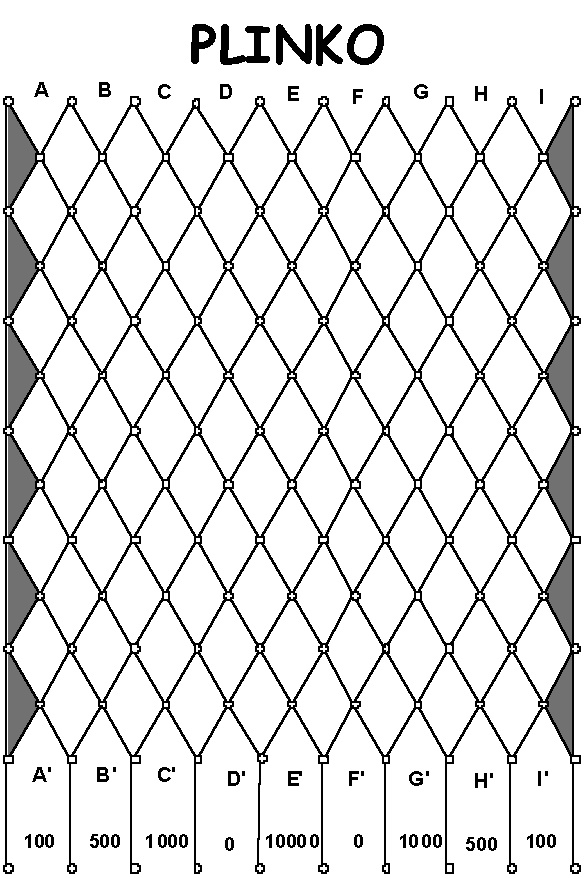
\includegraphics{board.jpg}

Image obtained from \href{http://www.mathdemos.org/mathdemos/plinko/}{http://www.mathdemos.org/mathdemos/plinko/}

Similar to previous examples, you  should have a series of trial simulations,
adding more and more disks to drop for each trial (on the Price is Right, contestants
drop from one to five disks).  You could start with five disks and double it
for each trial.  You will want to test what happens for each of the possible
slots that they can initially drop the disk, labeled as A through I in the above diagram.
The basic loop for simulating the trials would look like this:

\begin{Verbatim}[commandchars=\\\{\}]
\PYG{k}{while} \PYG{p}{(}\PYG{n}{numDisks} \PYG{o}{\PYGZlt{}} \PYG{n}{MAX}\PYG{p}{)} \PYG{p}{\PYGZob{}}
        \PYG{c+c1}{//drop numDisks thru each starting pos [A..I]}
        \PYG{n}{cout}\PYG{o}{\PYGZlt{}}\PYG{o}{\PYGZlt{}}\PYG{l+s}{"}\PYG{l+s+se}{\PYGZbs{}n}\PYG{l+s+se}{\PYGZbs{}n}\PYG{l+s}{Dropping }\PYG{l+s}{"} \PYG{o}{\PYGZlt{}}\PYG{o}{\PYGZlt{}} \PYG{n}{numDisks} \PYG{o}{\PYGZlt{}}\PYG{o}{\PYGZlt{}} \PYG{l+s}{"}\PYG{l+s}{ disks---}\PYG{l+s+se}{\PYGZbs{}n}\PYG{l+s}{"}\PYG{p}{;}
        \PYG{k}{for}\PYG{p}{(}\PYG{n}{pos}\PYG{o}{=}\PYG{l+s+sc}{'A'}\PYG{p}{;} \PYG{n}{pos}\PYG{o}{\PYGZlt{}}\PYG{o}{=}\PYG{l+s+sc}{'I'}\PYG{p}{;} \PYG{n}{pos}\PYG{o}{+}\PYG{o}{+}\PYG{p}{)} \PYG{p}{\PYGZob{}}
                \PYG{n}{dropDisks}\PYG{p}{(}\PYG{n}{pos}\PYG{p}{,} \PYG{n}{numDisks}\PYG{p}{,} \PYG{n}{numBigMoney}\PYG{p}{)}\PYG{p}{;}
        \PYG{p}{\PYGZcb{}}\PYG{c+c1}{//for-pos}

        \PYG{c+c1}{//show totals for this run...}
        \PYG{n}{showResults}\PYG{p}{(}\PYG{n}{numDisks}\PYG{p}{,} \PYG{n}{numBigMoney}\PYG{p}{)}\PYG{p}{;}

        \PYG{c+c1}{//increase \PYGZsh{}disks for next run}
        \PYG{n}{numDisks}\PYG{o}{+}\PYG{o}{=}\PYG{n}{numDisks}\PYG{p}{;}
\PYG{p}{\PYGZcb{}}\PYG{c+c1}{//while}
\end{Verbatim}

The function called \emph{dropDisks} would do the large task of trying each disk
to see where it lands.  The loop might look something like this:

\begin{Verbatim}[commandchars=\\\{\}]
\PYG{c+c1}{//The workhorse loop}
\PYG{k}{for} \PYG{p}{(}\PYG{n}{disk}\PYG{o}{=}\PYG{l+m+mi}{0}\PYG{p}{;} \PYG{n}{disk}\PYG{o}{\PYGZlt{}}\PYG{n}{numDisks}\PYG{p}{;} \PYG{n}{disk}\PYG{o}{+}\PYG{o}{+}\PYG{p}{)} \PYG{p}{\PYGZob{}}
        \PYG{k+kt}{double} \PYG{n}{valu} \PYG{o}{=} \PYG{n}{dropOneDisk}\PYG{p}{(}\PYG{n}{pos}\PYG{p}{)}\PYG{p}{;} \PYG{c+c1}{//how much did we win?}
        \PYG{n}{totalWon}\PYG{o}{+}\PYG{o}{=}\PYG{n}{valu}\PYG{p}{;}                 \PYG{c+c1}{//keep running total for pos}
        \PYG{k}{if} \PYG{p}{(}\PYG{n}{valu}\PYG{o}{=}\PYG{o}{=}\PYG{n}{BIG\PYGZus{}MONEY}\PYG{p}{)}    \PYG{c+c1}{//was it the BIG MONEY?}
                \PYG{n}{numBigMoneyHits}\PYG{o}{+}\PYG{o}{+}\PYG{p}{;}
\PYG{p}{\PYGZcb{}}\PYG{c+c1}{//for-disk}

\PYG{n}{numBigMoney}\PYG{p}{[}\PYG{n}{index}\PYG{p}{]}\PYG{o}{=}\PYG{n}{numBigMoneyHits}\PYG{p}{;}     \PYG{c+c1}{//tally bigMoney hits for pos}
\end{Verbatim}

As with the other examples presented earlier, using OpenMP to parallelize this loop
should be a fairly straightforward task.  The complex task for you is to code the logic
of the possible movement of the disks along each row and compute how often the
disk landed in each slot.


\section{Questions you could answer}
\label{Plinko/PlinkoGame:questions-you-could-answer}\begin{enumerate}
\item {} 
Where should I put my disks at the top to maximize the return at the bottom?

\item {} \begin{description}
\item[{For each starting slot, what is the probability that you will hit the big money slot?}] \leavevmode
Match your experimental results with the theoretical probabilities.

\end{description}

\end{enumerate}


\chapter{Exercises}
\label{NextSteps/Exercises:exercises}\label{NextSteps/Exercises::doc}
Here are example projects for you to try, now that you have run the previous examples.
\begin{enumerate}
\item {} 
Code the Monte Carlo method for approximating $\pi$ mentioned in the Introduction.  How many simulated dart throws do you need to run to approximate $\pi$ to 3 digits of accuracy?

\item {} 
Let's examine a twist on the example of drawing all four suits out of 5 drawn cards.  Write a program to shuffle a deck of cards and determine on average, how many cards you will need to draw:
\begin{enumerate}
\item {} 
before you have all four suits represented

\item {} 
before you get all four aces

\item {} 
before you get a \emph{marriage} (a King and Queen of the same suit)

\item {} 
before you get all 13 clubs

\item {} 
before your get a \emph{pinochle} (Queen of Spades and Jack of Diamonds)

\end{enumerate}

\item {} 
Given a system made of discrete components with known reliability, what is the reliability of the overall system? For example, suppose we have a system that can be described with the following high-level diagram:

\end{enumerate}

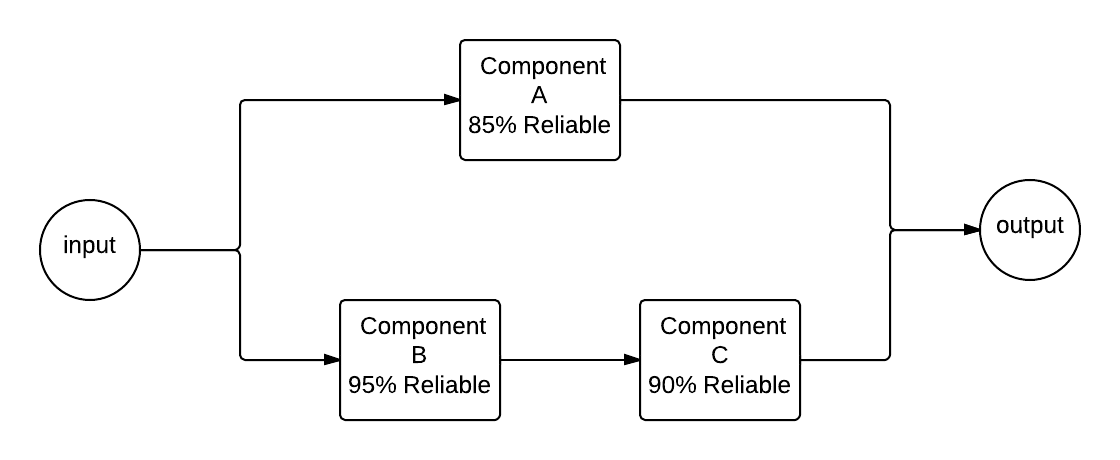
\includegraphics{StateDiagram.png}

When given an input to the system, that input flows through component A or through components B and C, each of which has a certain reliability of correctness.  Probability theory tells us the following:
\begin{gather}
\begin{split}reliability_{BC} = 0.95 * 0.90 = 0.855\end{split}\notag
\end{gather}\begin{gather}
\begin{split}reliability_A = 0.85\end{split}\notag
\end{gather}
And the overall reliability of the system is:
\begin{gather}
\begin{split}reliability_{sys} =  1.0 - [(1.0 - 0.85) * (1.0 - 0.855)]\end{split}\notag\\\begin{split}= 0.97825\end{split}\notag
\end{gather}
Create a simulation of this system where half the time the input travels through component A.  To simulate its reliability, generate a number between 0 and 1. If the number is 0.85 or below, component A succeeded, and the system works.  The other half of the time, the input would travel on the lower half of the diagram.  To simulate this, you will generate two numbers between 0 and 1.  If the number for component B is less than 0.95 and the number for component C is less than 0.90, then the system also succeeds.  Run many trials to see if you converge on the same reliability as predicted by probability theory.


\chapter{Advanced Topic:  Seeds For Different Threads}
\label{SeedingThreads/SeedEachThread::doc}\label{SeedingThreads/SeedEachThread:advanced-topic-seeds-for-different-threads}
Adding OpenMP pragmas on the `workhorse' for loops where most of the computation is being done is often a helpful way to make your code run faster.  In the case of Monte Carlo simulations, there is one issue that should be addressed to ensure the best random distribution of numbers from the random number generator functions.  We must start each thread with a different seed.

Recall that random number generators start from a `seed' large integer and create a sequence of integers by permuting the seed and each successive integer in a manner that ensures they are distributed across the range of all integers.  The key point is this: \emph{the sequence of numbers from a random generator is always the same when it starts with the same seed}.  In code where we fork threads to do the work of generating random numbers, we lose the desired random distribution if each thread begins generating random numbers from the same seed.

The solution to this issue for threaded code, which you can \code{download as coinFlip\_omp\_seeds.cpp}, is to ensure that each thread has its own seed from which it begins generating its sequence of integers.  Let's revisit the coin flipping example.  Instead of generating one seed in main using time(), we can save a seed for each thread in an array and devise a function to create all of the seeds, based on the number of threads to run.  We can add this code at the beginning of our original file:

\begin{Verbatim}[commandchars=\\\{\}]
\PYG{c+cm}{/***  OMP ***/}
\PYG{k}{const} \PYG{k+kt}{int} \PYG{n}{nThreads} \PYG{o}{=} \PYG{l+m+mi}{4}\PYG{p}{;}  \PYG{c+c1}{// number of threads to use}
\PYG{k+kt}{unsigned} \PYG{k+kt}{int} \PYG{n}{seeds}\PYG{p}{[}\PYG{n}{nThreads}\PYG{p}{]}\PYG{p}{;}

\PYG{k+kt}{void} \PYG{n}{seedThreads}\PYG{p}{(}\PYG{p}{)} \PYG{p}{\PYGZob{}}
    \PYG{k+kt}{int} \PYG{n}{my\PYGZus{}thread\PYGZus{}id}\PYG{p}{;}
    \PYG{k+kt}{unsigned} \PYG{k+kt}{int} \PYG{n}{seed}\PYG{p}{;}
    \PYG{c+cp}{\PYGZsh{}}\PYG{c+cp}{pragma omp parallel private (seed, my\PYGZus{}thread\PYGZus{}id)}
    \PYG{p}{\PYGZob{}}
        \PYG{n}{my\PYGZus{}thread\PYGZus{}id} \PYG{o}{=} \PYG{n}{omp\PYGZus{}get\PYGZus{}thread\PYGZus{}num}\PYG{p}{(}\PYG{p}{)}\PYG{p}{;}
        
        \PYG{c+c1}{//create seed on thread using current time}
        \PYG{k+kt}{unsigned} \PYG{k+kt}{int} \PYG{n}{seed} \PYG{o}{=} \PYG{p}{(}\PYG{k+kt}{unsigned}\PYG{p}{)} \PYG{n}{time}\PYG{p}{(}\PYG{n+nb}{NULL}\PYG{p}{)}\PYG{p}{;}
        
        \PYG{c+c1}{//munge the seed using our thread number so that each thread has its}
        \PYG{c+c1}{//own unique seed, therefore ensuring it will generate a different set of numbers}
        \PYG{n}{seeds}\PYG{p}{[}\PYG{n}{my\PYGZus{}thread\PYGZus{}id}\PYG{p}{]} \PYG{o}{=} \PYG{p}{(}\PYG{n}{seed} \PYG{o}{\PYGZam{}} \PYG{l+m+mh}{0xFFFFFFF0}\PYG{p}{)} \PYG{o}{\textbar{}} \PYG{p}{(}\PYG{n}{my\PYGZus{}thread\PYGZus{}id} \PYG{o}{+} \PYG{l+m+mi}{1}\PYG{p}{)}\PYG{p}{;}
        
        \PYG{n}{printf}\PYG{p}{(}\PYG{l+s}{"}\PYG{l+s}{Thread \PYGZpc{}d has seed \PYGZpc{}u}\PYG{l+s+se}{\PYGZbs{}n}\PYG{l+s}{"}\PYG{p}{,} \PYG{n}{my\PYGZus{}thread\PYGZus{}id}\PYG{p}{,} \PYG{n}{seeds}\PYG{p}{[}\PYG{n}{my\PYGZus{}thread\PYGZus{}id}\PYG{p}{]}\PYG{p}{)}\PYG{p}{;}
    \PYG{p}{\PYGZcb{}}
    
\PYG{p}{\PYGZcb{}}
\PYG{c+cm}{/***  OMP ***/}
\end{Verbatim}

Not how we change the seed value for each thread by using the thread's id to manipulate the original integer obtained from time().

Then later in the main function, we add a call to this function:

\begin{Verbatim}[commandchars=\\\{\}]
    \PYG{c+cm}{/***  OMP ***/} 
    \PYG{n}{omp\PYGZus{}set\PYGZus{}num\PYGZus{}threads}\PYG{p}{(}\PYG{n}{nThreads}\PYG{p}{)}\PYG{p}{;}  
    \PYG{n}{seedThreads}\PYG{p}{(}\PYG{p}{)}\PYG{p}{;}
    \PYG{c+cm}{/***  OMP ***/}
\end{Verbatim}

For each trial, we still parallelize the workhorse for loop, while also ensuring that each thread running concurrently has its own seed as the starting point for later numbers.

\begin{Verbatim}[commandchars=\\\{\}]
\PYG{c+cp}{\PYGZsh{}}\PYG{c+cp}{pragma omp parallel num\PYGZus{}threads(nThreads) default(none) \PYGZbs{}}
\PYG{c+cp}{        private(numFlips, tid, seed) \PYGZbs{}}
\PYG{c+cp}{        shared(trialFlips, seeds) \PYGZbs{}}
\PYG{c+cp}{        reduction(+:numHeads, numTails)}
    \PYG{p}{\PYGZob{}}
        \PYG{n}{tid} \PYG{o}{=} \PYG{n}{omp\PYGZus{}get\PYGZus{}thread\PYGZus{}num}\PYG{p}{(}\PYG{p}{)}\PYG{p}{;}   \PYG{c+c1}{// my thread id}
        \PYG{n}{seed} \PYG{o}{=} \PYG{n}{seeds}\PYG{p}{[}\PYG{n}{tid}\PYG{p}{]}\PYG{p}{;}            \PYG{c+c1}{// it is much faster to keep a private copy of our seed}
		\PYG{n}{srand}\PYG{p}{(}\PYG{n}{seed}\PYG{p}{)}\PYG{p}{;}	              \PYG{c+c1}{//seed rand\PYGZus{}r or rand}
        
        \PYG{c+cp}{\PYGZsh{}}\PYG{c+cp}{pragma omp for}
        \PYG{k}{for} \PYG{p}{(}\PYG{n}{numFlips}\PYG{o}{=}\PYG{l+m+mi}{0}\PYG{p}{;} \PYG{n}{numFlips}\PYG{o}{\PYGZlt{}}\PYG{n}{trialFlips}\PYG{p}{;} \PYG{n}{numFlips}\PYG{o}{+}\PYG{o}{+}\PYG{p}{)} \PYG{p}{\PYGZob{}}
\PYG{c+c1}{//          in Windows, can use rand()}
\PYG{c+c1}{//            if (rand()\PYGZpc{}2 == 0) // if random number is even, call it heads}
            \PYG{c+c1}{// linux: rand\PYGZus{}r() is thread safe, to be run on separate threads concurrently}
            \PYG{k}{if} \PYG{p}{(}\PYG{n}{rand\PYGZus{}r}\PYG{p}{(}\PYG{o}{\PYGZam{}}\PYG{n}{seed}\PYG{p}{)}\PYG{o}{\PYGZpc{}}\PYG{l+m+mi}{2} \PYG{o}{=}\PYG{o}{=} \PYG{l+m+mi}{0}\PYG{p}{)} \PYG{c+c1}{// if random number is even, call it heads}
                \PYG{n}{numHeads}\PYG{o}{+}\PYG{o}{+}\PYG{p}{;}       
            \PYG{k}{else}
                \PYG{n}{numTails}\PYG{o}{+}\PYG{o}{+}\PYG{p}{;}
        \PYG{p}{\PYGZcb{}}
        
    \PYG{p}{\PYGZcb{}}
\end{Verbatim}

Study the above code carefully and compare it to our first version below.  The \emph{pragma omp} directive above is forking the new set of threads, which do a bit of work to set up their own seeds.  Then the \emph{pragma omp for} directive is indicating that those same threads should now split up the work of the for loop, just as in our previous example using the OpenMP pragma.  The first OpenMP version we showed you looked like this:

\begin{Verbatim}[commandchars=\\\{\}]
\PYG{c+cp}{\PYGZsh{}}\PYG{c+cp}{pragma omp parallel for num\PYGZus{}threads(nThreads) default(none) \PYGZbs{}}
\PYG{c+cp}{        private(numFlips, seed) \PYGZbs{}}
\PYG{c+cp}{        shared(trialFlips) \PYGZbs{}}
\PYG{c+cp}{        reduction(+:numHeads, numTails)}
        \PYG{k}{for} \PYG{p}{(}\PYG{n}{numFlips}\PYG{o}{=}\PYG{l+m+mi}{0}\PYG{p}{;} \PYG{n}{numFlips}\PYG{o}{\PYGZlt{}}\PYG{n}{trialFlips}\PYG{p}{;} \PYG{n}{numFlips}\PYG{o}{+}\PYG{o}{+}\PYG{p}{)} \PYG{p}{\PYGZob{}}
            \PYG{c+c1}{// rand() is not thread safe in linux}
            \PYG{c+c1}{// rand\PYGZus{}r() is available in linux and thread safe,}
            \PYG{c+c1}{// to be run on separate threads concurrently.}
            \PYG{c+c1}{// On windows in visual studio, use rand(), which is thread safe.}
            \PYG{k}{if} \PYG{p}{(}\PYG{n}{rand\PYGZus{}r}\PYG{p}{(}\PYG{o}{\PYGZam{}}\PYG{n}{seed}\PYG{p}{)}\PYG{o}{\PYGZpc{}}\PYG{l+m+mi}{2} \PYG{o}{=}\PYG{o}{=} \PYG{l+m+mi}{0}\PYG{p}{)} \PYG{c+c1}{// if random number is even, call it heads}
                \PYG{n}{numHeads}\PYG{o}{+}\PYG{o}{+}\PYG{p}{;}       
            \PYG{k}{else}
                \PYG{n}{numTails}\PYG{o}{+}\PYG{o}{+}\PYG{p}{;}
        \PYG{p}{\PYGZcb{}}
\end{Verbatim}

\begin{notice}{note}{Note:}
A common `gotcha' that can cause trouble is if you accidentally use the original
\emph{pragma omp parallel for} directive near the for loop in the new version.  This causes     incorrect unintended behavior. Remember to remove the \textbf{parallel} keyword in the inner block when nesting bloaks as shown in the new version where we set up seeds first before splitting the loop work.
\end{notice}

Note that as before, in linux we need to use the rand\_r() function for thread-safe generation of the numbers.  However, in Windows, the rand() function is thread-safe.


\section{Try this yourself}
\label{SeedingThreads/SeedEachThread:try-this-yourself}
Try creating versions of the Roulette wheel simulation or drawing four suits that ensure that each thread is generating numbers from its own seed.



\renewcommand{\indexname}{Index}
\printindex
\end{document}
